\documentclass[journal]{IEEEtran}

\usepackage{cite,graphicx}
\usepackage[usenames,dvipsnames]{xcolor}

% *** GRAPHICS RELATED PACKAGES ***
%
\ifCLASSINFOpdf
  % \usepackage[pdftex]{graphicx}
  % declare the path(s) where your graphic files are
  % \graphicspath{{../pdf/}{../jpeg/}}
  % and their extensions so you won't have to specify these with
  % every instance of \includegraphics
  % \DeclareGraphicsExtensions{.pdf,.jpeg,.png}
\else
  % or other class option (dvipsone, dvipdf, if not using dvips). graphicx
  % will default to the driver specified in the system graphics.cfg if no
  % driver is specified.
  % \usepackage[dvips]{graphicx}
  % declare the path(s) where your graphic files are
  % \graphicspath{{../eps/}}
  % and their extensions so you won't have to specify these with
  % every instance of \includegraphics
  % \DeclareGraphicsExtensions{.eps}
\fi

\usepackage{graphicx}
\usepackage[cmex10]{amsmath}
\usepackage{algorithmic}
\usepackage{array}
\usepackage{mdwmath}
\usepackage{mdwtab}
\usepackage{eqparbox}
%\usepackage[tight,footnotesize]{subfigure}
%\usepackage[caption=false]{caption}
%\usepackage[font=footnotesize]{subfig}
%\usepackage[caption=false,font=footnotesize]{subfig}
\usepackage{fixltx2e}
\usepackage{stfloats}
\usepackage{url}

% *** Do not adjust lengths that control margins, column widths, etc. ***
% *** Do not use packages that alter fonts (such as pslatex).         ***
% There should be no need to do such things with IEEEtran.cls V1.6 and later.
% (Unless specifically asked to do so by the journal or conference you plan
% to submit to, of course. )

% correct bad hyphenation here
\hyphenation{op-tical net-works semi-conduc-tor}

\begin{document}
%
% paper title
% can use linebreaks \\ within to get better formatting as desired
\title{A Survey of Real-Time Strategy Game AI\\ Research and Competition in StarCraft}
%
%
% author names and IEEE memberships
% note positions of commas and nonbreaking spaces ( ~ ) LaTeX will not break
% a structure at a ~ so this keeps an author's name from being broken across
% two lines.
% use \thanks{} to gain access to the first footnote area
% a separate \thanks must be used for each paragraph as LaTeX2e's \thanks
% was not built to handle multiple paragraphs
%

% \author{FirstName~LastName,~\IEEEmembership{Member,~IEEE,}
%         Jim~Raynor,~\IEEEmembership{Fellow,~RR,}
%         and~Sarah~Kerrigan,~\IEEEmembership{Life~Fellow,~ZS}% <-this % stops a space
% \thanks{FirstName~LastName is with the Department of Names
% GA, 30332 USA e-mail: (see http://www.michaelshell.org/contact.html).}% <-this % stops a space
% \thanks{J. Raynor and S. Kerrigane are with the Romeo\&Juliet Inc.}% <-this % stops a space
% \thanks{Manuscript received April 19, 2499; revised January 11, 2500.}}

\author{Santiago~Onta\~{n}\'{o}n\thanks{Santiago~Onta\~{n}\'{o}n is with the Computer Science Department at Drexel University, Philadelphia, PA, USA.},
        Gabriel~Synnaeve\thanks{Gabriel~Synnaeve is with the Laboratory of Cognitive Science and Psycholinguistics (LSCP) of ENS Ulm in Paris, France.},
        Alberto~Uriarte\thanks{Alberto Uriarte is with the Computer Science Department at Drexel University, Philadelphia, PA, USA.},
        Florian~Richoux\thanks{Florian~Richoux is with the Laboratory of Computer Science of the University of Nantes, France.},
        David~Churchill\thanks{David~Churchill is with the Computing Science Department of the University of Alberta, Edmonton, Canada.},
        Mike~Preuss\thanks{Mike~Preuss is with the Department of Computer Science of Technische Universit{\"a}t Dortmund, Germany.}}



% note the % following the last \IEEEmembership and also \thanks - 
% these prevent an unwanted space from occurring between the last author name
% and the end of the author line. i.e., if you had this:
% 
% \author{....lastname \thanks{...} \thanks{...} }
%                     ^------------^------------^----Do not want these spaces!
%
% a space would be appended to the last name and could cause every name on that
% line to be shifted left slightly. This is one of those "LaTeX things". For
% instance, "\textbf{A} \textbf{B}" will typeset as "A B" not "AB". To get
% "AB" then you have to do: "\textbf{A}\textbf{B}"
% \thanks is no different in this regard, so shield the last } of each \thanks
% that ends a line with a % and do not let a space in before the next \thanks.
% Spaces after \IEEEmembership other than the last one are OK (and needed) as
% you are supposed to have spaces between the names. For what it is worth,
% this is a minor point as most people would not even notice if the said evil
% space somehow managed to creep in.

% The paper headers
\markboth{TCIAIG ~Vol.~X, No.~Y, Month~Year}%
{??? \MakeLowercase{\textit{et al.}}: A Survey of RTS Game AI Research and Competition in StarCraft}

\maketitle

\begin{abstract}
This paper presents an overview of the existing work on AI for real-time strategy (RTS) games. Specifically, we focus on the work around the game {\em StarCraft}, which has emerged in the past few years as the unified test-bed for this research. We describe the specific AI challenges posed by RTS games, and overview the solutions that have been explored to address them. Additionally, we also present a summary of the results of the recent StarCraft AI competitions, describing the architectures used by the participants. Finally, we conclude with a discussion emphasizing which problems in the context of RTS game AI have been solved, and which remain open.
\end{abstract}

\begin{IEEEkeywords}
Game AI, Real-Time Strategy, StarCraft, Review1

\end{IEEEkeywords}

% For peer review papers, you can put extra information on the cover
% page as needed:
% \ifCLASSOPTIONpeerreview
% \begin{center} \bfseries EDICS Category: 3-BBND \end{center}
% \fi
%
% For peerreview papers, this IEEEtran command inserts a page break and
% creates the second title. It will be ignored for other modes.
\IEEEpeerreviewmaketitle

\section{Introduction}\label{sec:intro}
\IEEEPARstart{T}{he} field of real-time strategy (RTS) game AI has advanced significantly since Michael Buro's call for research in this area \cite{Buro03rts}. Specially, competitions like the ``AIIDE StarCraft AI Competition'' have motivated the exploration of many AI approaches in the context of RTS AI. We will list and classify these approaches, explain their 
strengths and weaknesses and conclude on what is left to achieve human-level 
RTS AI.

Complex dynamic environments, where it is not possible to have neither perfect nor complete information about the current state or about the dynamics of the environment, pose significant challenges for artificial intelligence. Road  traffic, finance, or
weather  forecasts are  examples of such large, complex, real-life dynamic
environments. RTS games can be seen as a simplification of one such real-life
environment, with simpler dynamics in a  finite and smaller
world, although still complex enough  to study some of the key interesting
problems like decision making  under
uncertainty  or  real-time adversarial planning. Finding efficient  techniques for
tackling  these problems  on  RTS  games can  thus  benefit other AI disciplines and application
domains, and also have concrete  and direct applications in  the ever growing
industry of  video games.%, generating worldwide two  and a  half times more revenue than the Film industry in 2011.
% This statement is not fair, the reference I found it only compare all the game industry revenue (including hardware sales) vs theatrical film industry revenue (i.e. not DVD sales, ...)

This paper aims to provide a one-stop guide on what is the state of
the art in RTS AI, with a particular emphasis on the work done in StarCraft. 
It is organized as follows: Section~\ref{sec:rts}
introduces RTS games, in particular the game StarCraft,
and  their main  AI challenges.  Section~\ref{sec:review}
reviews  the existing  work on tackling these challenges in RTS games.
Section~\ref{sec:bot} analyzes several current state of the art RTS game playing agents (called {\em bots}), selected form the participants to annual
StarCraft    AI    competitions.
Section~\ref{sec:competition}  presents results of the recent annual competitions
held at the AIIDE  and CIG conferences and a StarCraft bot game ladder\footnote{An extended tournament, which can potentially go on indefinitely.}.  Section~\ref{sec:questions}
compiles open questions in RTS game AI. Finally, the paper concludes on discussions and perspectives.

% {\color{blue}
% Motivate the paper, and provide an outline.

% Some arguments to use in the motivation could be that games are a good application to motivate novel AI research (as has been happening throughout the history of AI), and that techniques and algorithms developed for RTS games, in addition to be useful and relevant to the game industry, have broader application to other areas.

% Reiterate that the goal of this paper is to provide a one-stop guide on what is the
% state of the art in StarCraft AI
% }

\section{Real-Time Strategy Games}\label{sec:rts}

Real-time Strategy (RTS) is a sub-genre of strategy games where players need to build an economy (gathering resources and building a base) and military power (training units and researching technologies) in order to defeat their opponents (destroying their army and base). From a theoretical point of view, the main differences between RTS games and traditional board games such as Chess are:

\begin{itemize}
\item They are {\em simultaneous move} games, where more than one player can issue actions at the same time. Additionally, these actions are {\em durative}, i.e. actions are not instantaneous, but take some amount of time to complete.
\item RTS games are ``real-time'', which actually means is that each player has a very small amount of time to decide the next move. Compared to Chess, where players may have several minutes to decide the next action, in StarCraft, the game executes at 24 iterations per second, which means that players can act as fast as every 42ms, before the game state changes.
\item Most RTS games are partially observable: players can only see the part of the map that has been explored. This is referred to as the {\em fog-of-war}.
\item Most RTS games are non-deterministic. Some actions have a chance of success.
\item And finally, the complexity of these games, both in terms of state space size and in terms of number of actions available at each decision cycle is very large. For example, the state space of Chess is typically estimated to be around $10^{50}$, heads up no-limit Texas holdem poker around $10^{80}$, and Go around $10^{170}$. In comparison, the state space of StarCraft in a typical map is estimated to be many orders of magnitude larger than any of those, as discussed in the next section.
\end{itemize}

For those reasons, standard techniques used for playing classic board games, such as game tree search, cannot be directly applied to solve RTS games without the definition of some level of abstraction, or some other simplification. Interestingly enough, humans seem to be able to deal with the complexity of RTS games, and are still vastly superior to computers in these types of games \cite{burochurchill2012aimagazine}. For those reasons, a large spectrum of techniques have been attempted to deal with this domain, as we will describe below. The remainder of this section is devoted to describe StarCraft as a research testbed, and on detailing the open challenges in RTS game AI.

\subsection{StarCraft}\label{subsec:StarCraft}

{\em StarCraft: Brood War} is an immensely popular RTS game released in 1998 by Blizzard Entertainment. StarCraft is set in a science-fiction based universe where the player must choose one of the three races: Terran, Protoss or Zerg. One of the most remarkable aspects of StarCraft is that the three races are extremely well balanced:

\begin{itemize}
	\item Terrans, provide units that are versatile and flexible giving a balanced option between Protoss and Zergs.
	\item Protoss units have lengthy and expensive manufacturing process, but they are strong and resistant. These conditions make players follow a strategy of quality over quantity.
	\item Zergs, the insectoid race, units are cheap and weak. They can be produced fast, encouraging players to overwhelm their opponents with sheer numbers.
\end{itemize}


Figure~\ref{fig:StarCraft} shows a screenshot of StarCraft showing a player playing the Terran race. In order to win a StarCraft game, players must first gather resources (minerals and Vespene gas). As resources become available, players need to allocate them for creating more buildings (which reinforce the economy, and allow players to create units or unlock stronger units), research new technologies (in order to use new unit abilities or improve the units) and train attack units. Units must be distributed to accomplish different tasks such as reconnaissance, defense and attack. While performing all of those tasks, players also need to strategically understand the geometry of the map at hand, in order to decide where to place new buildings (concentrate in a single area, or expand to different areas) or where to set defensive outposts. Finally, when offensive units of two players meet, each player must quickly maneuver each of the units in order to fight a battle, which requires quick and reactive control of each of the units.

\begin{figure}
    \centering
    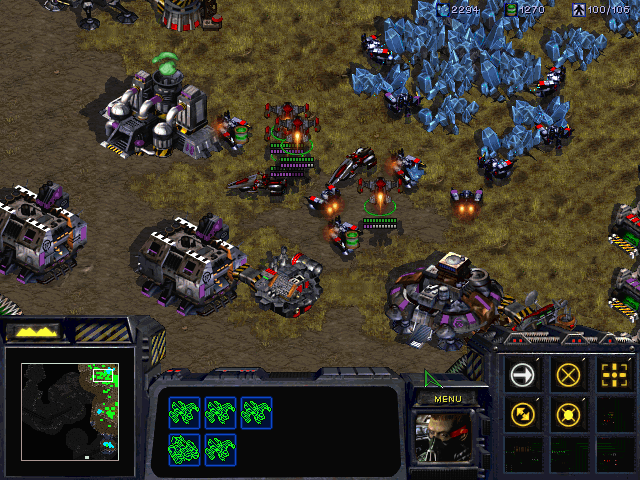
\includegraphics[width=0.8\columnwidth]{figures/starcraft1.png}
    \caption{A screenshot of \emph{StarCraft: Brood War}% {\color{red} is this a good screenshot? can we actually have a screenshot? or is this copyrighted? Do we even want a screenshot?}.
    .}
    \label{fig:StarCraft}
\end{figure}

A typical StarCraft map is defined as a rectangular grid, where the $width \times height$ of the map is measured in the number of $32 \times 32$ square of pixels, also known as build tiles. Although the
resolution of walkable areas is in squares of $8 \times 8$ pixels, also known as walk tiles. The typical dimensions for maps range from $64 \times 64$ to $256 \times 256$ build tiles. Each player  can
control up  to 200 units (plus an unlimited number of buildings).  Moreover, each
different race  contains between 30  to 35 different types  of units
and  buildings,  most of them with  a significant  number  of  special
abilities. All these factors  together make StarCraft a significant
challenge,   in   which   humans    are   still   much   better   than
computers. For instance, in the game ladder iCCup\footnote{http://www.iccup.com/StarCraft/} where users are ranked by their current point totals ($E$ being the lowest possible rank, and $A^+$ and $Olympic$ being the second highest and highest ranks, respectively), the best StarCraft AI bots are ranked between $D$ and $D^+$, where average  amateur players are  ranked between $C^+$ and  $B$. For comparison, StarCraft professional  players are usually ranked between
$A^-$ and $A^+$.

From a theoretical point of view, the state space of a StarCraft for a given map is enormous. For example, consider a $128 \times 128$ map. At any given moment there might be between 50 to 400 units in the map, each of which might have a complex internal state (remaining energy and hit-points, action being executed, etc.). This quickly leads to an immense number of possible states (way beyond the size of smaller games, such as Chess or Go). For example, just considering the location of each unit (with $128 \times 128$ possible positions per unit), and 400 units, gives us an initial number of $16384^{400} \approx 10^{1685}$. If we add the other factors playing a role in the game, we obtain even larger numbers. 

Another way  to measure the complexity  of the game is  by looking at
the branching factor, $b$, and the depth of the game, $d$, as proposed in~\cite{Gaby}, with a total game complexity of $b^d$. In Chess, $b \approx 35$ and $d \approx 80$. In more complex games, like Go, $b \approx 30 - 300$, and $d \approx 150 - 200$. In order to determine the branching factor in StarCraft when an AI plays it, we must have in mind, that the AI can issue actions simultaneously to as many units in the game as desired. Thus, considering that, in a typical game, a player controls between 50 to 200 units, the branching factor would be between $u^{50}$ and $u^{200}$, where $u$ is the number of actions each unit can execute. Assuming a conservative value for $u$ of about $30$ (moving to nearby positions, attacking units in range, using special abilities, etc.), we obtain a branching factor of $b$ between  $30^{50}$ and $30^{200}$. Now, to compute $d$, we simply consider the fact that typical games last for about 25 minutes, which results in $d \approx 36000$ (25 minutes $\times$ 60 seconds $\times$ 24 iterations per second).

%In StarCraft, humans can issue only one action at a time (this is because of the GUI used by the game, computer players can issue several actions, to different units, at any given time), thus, assuming a player controls between 50 to 200 units, and that each unit can execute between 4 to 20 actions (moving in each of the 4 cardinal directions, attacking units in range, use special abilities, etc.), we estimate the branching factor for human players to be around $b \approx 200 - 4000$. Good players can execute about 300 actions per minute, and the typical length of a game is about 25 minutes. Thus, $d \approx 7500$.

%However, this is a weak indication of the complexity of the game, since many of those states would never be reached in a game. For that reason, it is more useful to just think in terms of the branching factor and depth of a game, when a human plays it. In Chess, the branching factor is around 35 and the depth, around 80. In Go, the branching factor is between 30 to 300 and the depth 150 to 200. In StarCraft, humans can execute about ...


% From Gabriel's dissertation:
% ------------------------------------
%ÒHow does the state of possible actions grow?Ó To measure this, we
%used a measure from perfect information zero-sum games (as Checkers,
%Chess and Go): the branching factor* b and the depth d of a typical
%game. The complexity of a game (for taking a decision) is proportional
%to bd.
%[...]
%In RTS games, b Å 200 is a lower bound (in StarCraft we may have
%between 50 to 400 units to control), and very good amateurs and
%professional players perform more than 300 actions per minute. As
%StarCraft is a simultaneous move, multi-units game, a strict number
%for b would be |actions||units| (actions account for atomic moves and
%abilities), thus for StarCraft b would be around 30^{60}. Strictly
%speaking, for a StarCraft game, d = 24  game_seconds (24 game frames
%per second), with a game duration of 25 minutes, this gives d Å
%36,000, thus b^d Å 30^{60^{36000}} .



\subsection{Challenges in RTS Game AI}\label{subsec:challenges}

Early research in AI for RTS games \cite{Buro03rts} identified the following six challenges: 
\begin{itemize}
\item Resource management
\item Decision making under uncertainty
\item Spatial and temporal reasoning
\item Collaboration (between multiple AIs)
\item Opponent modeling and learning
\item Adversarial real-time planning
\end{itemize}

While there has been a significant work in many, others have been untouched (e.g. collaboration). Moreover, recent research in this area has identified several additional research challenges, such as how to exploit the massive amounts of existing domain knowledge (strategies, build-orders, replays, and so on). Below, we describe current challenges in RTS Game AI, grouped in six main different areas.

%\begin{itemize}
%\item Task Decomposition (or ``Architecture'')
%\item Integration of Domain Knowledge
%\item Reasoning with Uncertainty (including information gathering)
%\item Opponent Modeling and Adaptation: opponent modeling is key if we have to adapt our strategy. As different strategies are dominating each others, forming multiple Nash equilibria, the AI has to be able to infer the intend of its opponent.
%\item Group and Individual Control (``micro''): the task of controlling units efficiently (we can not speak of optimality here due to the huge state space, and of the enemy behavior entails numerous Nash equilibria), focusing fire to diminish enemy's firepower and keeping our units alive the longest, casting defensive and offensive spells and abilities.
%\item Planning and Resource Allocation (``macro'')
%\item Spatial reasoning (``tactics'')
%\end{itemize}

\subsubsection{Planning}
As mentioned above, the size of the state space in RTS games is much larger than that of traditional board games such as Chess or Go. Additionally, the number of actions that can be executed at a given instant of time is also much larger. Thus, standard adversarial planning approaches, such as game tree search are not directly applicable. As we elaborate later, planning in RTS games can be seen as having multiple levels of abstraction: at a higher level, players need long-term planning capabilities, in order to develop a strong economy in the game; at a low level, individual units need to be moved in coordination to fight battles taking into account the terrain and the opponent. Techniques that can address these large planning problems by either sampling, or hierarchical decomposition do not yet exist.

\subsubsection{Learning}
Given the difficulties in playing RTS games by directly using adversarial planning techniques, many research groups have turned attention to learning techniques. We can distinguish three types of learning problems in RTS games:
\begin{itemize}
\item {\em Prior learning}: How can we exploit available data, such as existing replays, or information about specific maps for learning appropriate strategies before hand? A significant amount of work has gone in this direction.%, such as \cite{WeberCIG09,SynnaeveCIG11,SynnaeveAIIDE11,OntanonMSR10}.
\item {\em In-game learning}: How can bots deploy online learning techniques that allow them to improve their game play while playing a game? These techniques might include reinforcement learning techniques, but also opponent modeling. The main problem again is the fact that the state space is too large and the fact that RTS games are partially observable.
\item {\em Inter-game learning}: What can be learned from one game that can be used to increase the chances of victory in the next game? Some work has used simple game-theoretical solutions to select amongst a pool of predefined strategies, but the general problem remains unsolved.
\end{itemize}

%%% I think there are two important aspects of uncertainty in RTS games:
%%% \begin{itemize}
%%% \item First is trying to model uncertainty and try to reduce it (information gathering, and representation of knowledge), this includes scouting, and maintaining good estimates of locations and number of units of the enemy, etc.
%%% \item Second is actually using the uncertain information. Taking decisions like army strength estimation (like to attack or retreat).
%%% \end{itemize}

\subsubsection{Uncertainty}
Adversarial planning under uncertainty in domains of the size of RTS games is still an unsolved challenge.
In RTS games, there are two main kinds of uncertainty. First, the game is partially observable, and players cannot observe the whole game map (like in Chess), but need to scout in order to see what the opponent is doing. This type of uncertainty can be lowered by good scouting, and knowledge representation (to infer what is possible given what has been seen). Second, there is also uncertainty arising from the fact that the games are adversarial, and a player cannot predict the actions that the opponent(s) will execute. For this type of uncertainty, the AI, as the human player, can only build a sensible model of what the opponent is likely to do. 
% [Santi: I commented out this part, since I'm not sure it's correct. The second type of uncertainty can also be linked to data. For example, by analyzing player replays, one could learn "plan recognition" probability tables, which can be used to infer the strategy of the opponent, and thus, reduce the uncertainty of the opponent's future actions]
%Both these kinds of uncertainty can be studied through probabilities, but only the first type, $P(Hidden | Seen)$, can be {\em easily} linked to data. %now for the clumsy part:
%One could argue that the extensional data is the only thing that matters because it is the only thing that has an influence on the game, but in reality, for very highly skilled players, discovering the intentions of the enemy is the key to winning. It allows for a compact understanding of the game state and development, while also giving additional information about the future. Whereas a player is doing action A to follow it up by action B or C depends on its intention, while the information about action A is visible and information about B or C is hidden, only intention allows for a choice.

\subsubsection{Spatial and Temporal Reasoning}
% TODO just a paragraph on exposing why there are temporal and spatial
% reasoning in RTS AI.
Spatial  reasoning   is  related  to   each  aspect  of   terrain
exploitation.  Spatial reasoning is involved in tasks such as building placing, or base expansion. In the former, the player needs to
carefully  consider building  position  into its  own  bases to  both
protect them  by creating  a wall against  invasions and to  avoid bad
configurations  where large  units could  be stuck. In base expansion, the player has to
choose good available locations to  build a new base, regarding its
own  position  and opponent's  bases.  Finally,  spatial reasoning  is
key to tactical reasoning: players need to decide where to place units
for battle,  favoring, for  instance, engagements when  the opponent's
units are into a bottleneck. 

% [Flo:  70% to hit high  ground units according to  Ben Weber's paper
% [3], and 53.125% according  to BWAPI website. Who's right? Should we
% add this in the paper?]
% [Alberto: I guess Weber's number comes from StarCraft walkthroughs like this: http://www.supercheats.com/pc/walkthroughs/starcraftbroodwar-walkthrough01.txt, there is also a chance to hit in even grounds (like 98%). But since we cannot see the original code all of these numbers are approximations. In any case we can keep explaining the concept without numbers ;)]
Another example of spatial reasoning in StarCraft is that it is always an advantage to  have its units  on high ground  while enemy is on low ground, since units  on low ground have no vision  on high ground, and firing from low ground have a chance to  hit units on high ground.

Analogously, temporal reasoning is key in tactical or strategic reasoning. For example, timing attacks and retreats to gain advantage. At a higher strategic level, players need to reason about when to perform long-term impact economic actions such as upgrades, building construction, strategy switching, etc. all taking into account that the effects of these actions are not immediate, but longer term.


\subsubsection{Domain Knowledge Exploitation}
In traditional board games such as Chess, researchers have exploited the large amounts of existing domain knowledge to create good evaluation functions to be used by alpha-beta search algorithms, extensive opening books, or end-game tables. In the case of RTS games, it is still unclear the ways in which the significantly large amount of domain knowledge (in the forms or strategy guides, replays, etc.) can be exploited by bots. Most work in this area has focused on two main directions: on the one hand, researchers are finding ways in which to hard-code existing strategies into bots, so that bots only need to decide which strategies to deploy, instead of having to solve the complete problem of deciding which actions to execute by each individual unit at each time step. One the other hand, large datasets of replays have been created \cite{WeberCig09,synnaeve2012dataset}, from where strategies, trends or plans have been tried to learn. However, StarCraft games are quite complex, and how to automatically learn from such datasets is still an open problem.

\subsubsection{Task Decomposition}
For all the previous reasons, most existing approaches to play games like StarCraft work by decomposing the problem of playing a RTS game into a collection of smaller problems, to be solved independently. Specifically, a common subdivision is:
\begin{itemize}
\item {\em Strategy}: corresponds to the high-level decision making process.  This is
  the  highest level of  abstraction for  the game  comprehension. Finding   an   efficient   strategy   or
  counter-strategy  against a  given opponent is key in RTS games.  It concerns  the whole
  set of  units and buildings  a player owns. %If  we may allow  ourselves a  military analogy, strategy is orders given by generals at the HQ. 
\item  {\em Tactics}: are  the implementation  of the  current  strategy. It
  implies  army and  building positioning,  movements, timing,  and so
  on.  Tactics concerns a  group of  units. %They  are orders  given by officers on the battlefield.
\item  {\em Reactive  control}: is  the  implementation  of  tactics.  This
  consists   in  moving,   targeting,  firing,   fleeing,  hit-and-run
  techniques (also knows as ``kiting'')  during battle. Reactive control focuses
  on a specific unit. %It is soldiers applying officers' orders. 
%\end{itemize}
%
%\noindent
%Both     strategy      and     tactics     are      usually     called
%\textit{macro-management},  whereas reactive  control  is also  called
%\textit{micro-management}. In addition of the three tasks shown above,
%one could also consider these two tasks that an AI has to deal with:
%\begin{itemize}
\item {\em Terrain analysis}: consists  in the analysis of regions composing
  the  map:  choke-points,  minerals  and  gas emplacements,  low  and  high
  walkable grounds, islands, etc.
\item {\em Intelligence gathering}:  corresponds to information collected about
  the  opponent. Because of  the fog-of-war,  players must
  regularly send scouts to localize and spy enemy bases.%, and must see or  infer what buildings and technology the enemy has developed in order  to adapt its strategy.
\end{itemize}

In comparison, when humans play StarCraft, they typically divide their decision making in a very different way. The StarCraft community typically talks about two tasks:
\begin{itemize}
  \item {\em Micro}: is the ability to control your units individually. A good \emph{micro} player usually keeps their units alive during more time.
  \item {\em Macro}: is the ability to produce units and to expand at the appropriate times to keep your production of units flowing. A good \emph{macro} player usually has the larger army.
\end{itemize}

The reader can find a  good presentation of task decomposition for AIs
playing RTS in~\cite{weber2011acs}. Although the previous task decomposition is common, a significant challenge is on designing architectures so that the individual AI techniques that address each of those tasks can communicate and effectively work together, resolving conflicts, prioritizing resources between them, etc. Section \ref{sec:bot} provides an overview of the task decompositions that state-of-the-art bots use.


\section{Existing work on RTS Game AI}\label{sec:review}

\begin{figure}
    \centering
    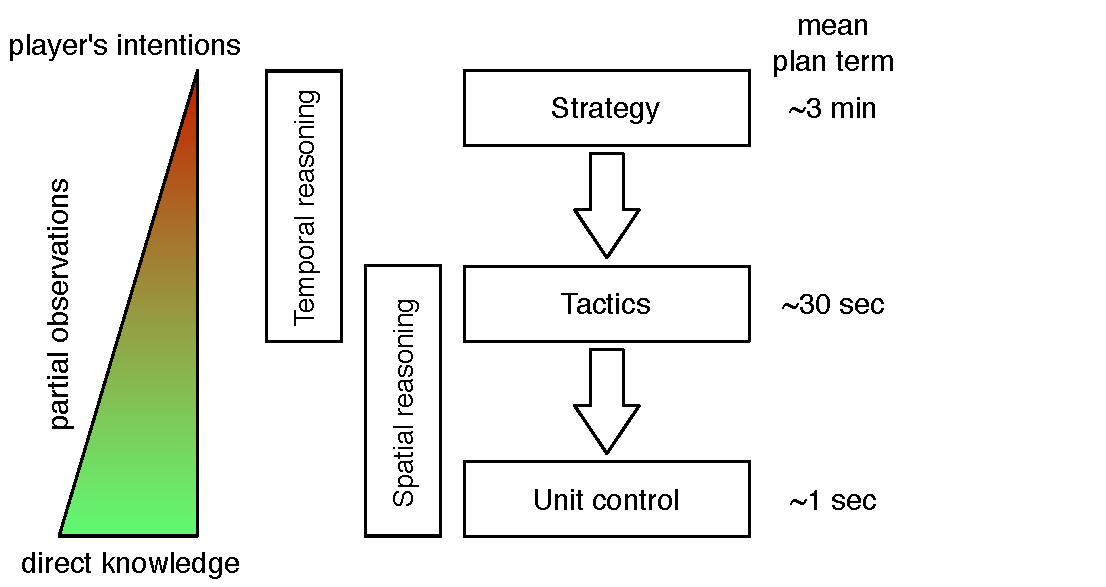
\includegraphics[width=0.9\columnwidth]{figures/levels_abstraction.pdf}
    \caption{RTS AI levels of abstraction and their properties: uncertainty (from intentions and from partial observation) is going higher as the abstraction levels are raising. The timings on the right correspond to an estimate of the duration of a behavior switch in StarCraft. Spatial and temporal reasoning are indicated for part for which greedy solutions are really not efficient.}
    \label{fig:levels-abstraction}
\end{figure}

Systems that play RTS games need to address most, if not all, the aforementioned problems together. Therefore, it is hard to classify existing work on RTS AI as addressing the different problems above. For that reason, in order to classify existing work on RTS AI, we will divide it according to three levels of abstraction: strategy (which loosely corresponds to ``macro''), tactics and reactive control (which loosely corresponds to ``micro''). 

Figure~\ref{fig:levels-abstraction} graphically illustrates how strategy, tactics and reactive control are three points in a continuum scale where strategy corresponds to decisions making processes that affect long spans of time (several minutes in the case of StarCraft), reactive control corresponds to low-level second-by-second decisions, and tactics sit in the middle. Also, strategic decisions reason about the whole game at once, whereas tactical or reactive control decisions are localized, and affect only specific groups of units. Typically, strategic decisions constraint future tactical decisions, which in turn condition reactive control. Moreover, information gathered while performing reactive control, can cause reconsideration of the tactics being employed; which could trigger further strategic reasoning.

Following this idea, we consider strategy to be everything related to the technology trees, build-order\footnote{The {\em build-order} is the specific sequence in which buildings of different types will be constructed at the beginning of a game, and completely determines the long-term strategy of a player.}, upgrades, and army composition. It is the most deliberative level, as a player selects and performs a strategy with future stances (aggressive, defensive, economy, technology) and tactics in mind. We consider tactics to be everything related to confrontations between groups of units. Tactical reasoning involves both spatial (exploiting the terrain) and temporal (army movements) reasoning, constrained on the possible types of attacks by the army composition of the player and their opponent. Finally, we will call reactive control to how the player controls individual units to maximize their efficiency (when executing tactics) in real-time. The main difference between tactics and reactive control is that tactical reasoning typically involves some sort of planning ahead for some short spans of time, whereas reactive control involves no planning ahead whatsoever.

% Example:
For example, after starting a game, a player might decide to use a {\em rushing} strategy (which involves quickly building an army and sending it to attack as early as possible in the game); then, when performing the attack use a {\em surrounding} tactic, where the player tries to surround the enemy cutting potential escape routes; finally, while executing the surrounding tactic, the player might decide to use reactive control techniques that command individual units to perform repeated {\em attack and flee} movements, to maximize the efficiency of each of the units being used in the attack.

%{\color{blue}
%perhaps TODO ``how it's done in the industry'' regrouping the first paragraph of each of the following 3 sections?
%}


\subsection{Strategy}
%Every AI needs to observe the world in order to analyze it and take decisions. In RTS games this task isn't trivial since we have to deal with imperfect information.
%The most common decision making are Decision Trees. Some of the advantages of the decision trees are: simple to understand and interpret acting like a white box where we can explain why a decision is taken, and they are compatible with other decision techniques. For complex decisions we have many algorithms to generate an optimum decision tree like ID3 or C4.5, depends on the problem we will use one or another.

% INTRO:
Strategic decision making in real-time domains is still an open problem. In the context of RTS games is has been addressed using many AI techniques, like hard-coded approaches, planning-based approaches, or machine learning-based approaches. We cover each of these approaches in turn.

% HARD-CODED:
Hard-coded approaches have been extensively used in commercial RTS games. The most common approaches use finite state machines (FSM) \cite{FSM_AIGameProgWisdom2003} in order to let the AI author hard-code the strategy that the AI will employ. The idea behind FSMs is to decompose the AI behavior into easily manageable states, such as ``attacking'', ``gathering resources'' or ``repairing'' and establish the conditions that trigger transitions between them. Commercial approaches also include Hierarchical FSMs, in which FSMs are composed hierarchically. These hard-coded approaches have achieved a significant amount of success, and, as we will discuss later, have also been used in many academic RTS AI research systems, as discussed in Section \ref{sec:bot}. However, these hard-coded approaches struggle to encode dynamic, adaptive behaviors, and are easily exploitable by adaptive opponents.

% XXX: Santi: I've commented out this paragraph, since it has nothing to do with RTS games. There is no commercial RTS game using planning (neither STRIPS nor HTN) that I'm aware of. The references below refer to FEAR, which is an FPS game.
%To this end, several approaches have been developed like hierarchical task networks, behavior trees and the comeback of STRIPS \cite{FikesSTRIPS} planning in the industry \cite{orkinGDC_FEAR}. Regardless, one cannot but notice that adaptability is not the strong point of industrial RTS AI. In the context of RTS AI strategy adaptation is related to the idea of opponent modeling. An adapting AI needs to keep track of what the enemy is doing in order to estimate the probability that they will use a specific strategy and adapt its own strategy accordingly. 


% PLANNING:
Approaches using planning techniques have also been explored in the literature. For example Onta\~{n}\'{o}n et al. \cite{CBR_Planning} explored the use of real-time case-based planning (CBP) in the domain of Wargus (a Warcraft II clone). In their work, they used human demonstration to learn plans, which are then composed at run-time in order to form full-fledges strategies to play the game. In \cite{PlanRetrieval} they improve over  their previous CBP approach by using situation assessment for improving the quality and speed of plan retrieval. Hierarchical Task-Network (HTN) planning has also been explored with some success in the context of simpler first-person shooter games \cite{HTNPlanning}. Planning approaches offer more adaptivity of the AI strategy compared to hard-coded approaches. However, the real-time constraints of RTS games limit the planning approaches that can be applied, being HTN and case-based planning the only ones explored so far. Moreover, none of these approaches addresses any timing or scheduling issues, which are key in RTS games. On notable exception is the work of Churchill and Buro \cite{churchill2011build}, who used planning in order to construct its economic build-orders taking into account timing constraints of the different actions.

% MACHINE LEARNING:
Concerning machine learning-based approaches, Weber and Mateas \cite{WeberCig09} proposed a data mining approach to strategy prediction and performed supervised learning on labeled StarCraft replays. Dereszynski et al. \cite{HMMstrat_RTS_AIIDE11} used Hidden Markov Models (HMM) to learn the transition probabilities of sequences of building construction orders and kept the most probable ones to produce probabilistic behavior models (in StarCraft). Synnaeve and Bessi\`{e}re \cite{SynnaeveOpeningCig11} used the dataset of \cite{WeberCig09} and presented a Bayesian semi-supervised model to learn from replays and predict openings (early game strategies) from StarCraft replays. The openings are labeled by EM clustering considering appropriate features. Then, in \cite{SynnaeveAIIDE11}, they presented an unsupervised learning Bayesian model for tech-tree prediction, still using replays. % Finally \cite{GemineImitative} used the same ``build-order features'' approach to learn to adapt the bot's build order to the opponents strategy in StarCraft 2.
Finally, evolutionary approaches to determine priorities of high level tasks was explored by Young and Hawes in their QUORUM system \cite{young2012evolutionary}, showing improvement over static priorities.

% CBR:
Also falling into the machine-learning category, a significant group of researchers has explored case-based reasoning (CBR) \cite{Aamodt94CBR} approaches for strategic decision making. For example Aha et al. \cite{LTW} used CBR to perform dynamic plan retrieval in the Wargus domain. Hsieh and Sun \cite{HsiehS08} based their work on Aha et al.'s CBR model \cite{LTW} and used StarCraft replays to construct states and building sequences (``build orders''). Finally, Schadd et al. \cite{SchaddBS07} applied a CBR approach to opponent modeling through hierarchically structured models of the opponent behavior and they applied their work to the Spring RTS game (a ``Total Annihilation'' clone).

% SCOUTING:
One final consideration concerning strategy is that RTS games are typically partially observable. Games like StarCraft implement the ``fog-of-war'' idea, which basically means that a player can only see the areas of the map close to her own units. Areas of the map away from the field of view of individual units are not observable. Players need to scout in order to obtain information about the opponent's strategy. The size of the state space in StarCraft prevents solutions based on POMDPs from being directly applicable, and very few of the previous approaches deal with this problem. Most research in RTS game AI assumes perfect information all the time, this mean that they only consider the information that they can see to make decisions. In the case of commercial games, most AI implementations cheat, since they have perfect information, while the human player does not. In order to make the human player believe the AI of these games does not cheat, sometimes they simulate some scouting tasks as Bob Fitch described in his AIIDE 2011 keynote for the WarCraft and StarCraft game series. A notable exception is the work of Weber et al. \cite{WeberAIIDE11}, who used a particle model with a linear trajectory update to track opponent units under fog-of-war in StarCraft. They also produced tactical goals through reactive planning and goal-driven autonomy \cite{WeberCig10,Weber10}, finding the more relevant goal(s) to spawn in unforeseen situations. 


\subsection{Tactics}

% INTRO:
Tactical reasoning involves reasoning about the different abilities of the units in a group and about the environment (terrain) and positions of the different groups of units in order to gain military advantage in battles. For example, it would be a very bad tactical decision to send fast, invisible or flying units (typically expensive) in the first line of fire against slower heavier units, since they will be wiped out fast. We will divide the work on tactical reasoning in two parts: terrain analysis and decision making.

% TERRAIN ANALYSIS:
Terrain analysis supplies the AI with structured information about the map in order to help making decisions. This analysis is usually performed off-line, in order to save CPU time during the game. For example, Pottinger \cite{Pottinger00} described the \emph{BANG} engine implemented by Ensemble Studios for the game Age of Empires II. This engine provides terrain analysis functionalities to the game using influence maps and areas with connectivity information. 
Forbus et al. \cite{Forbus2002} showed the importance to have qualitative spatial information for wargames, for which they used geometric and pathfinding analysis. 
Hale et al. \cite{Hale08} presented a 2D geometric navigation mesh generation method from expanding convex regions from seeds. 
Finally, Perkins \cite{Perkins10} applied Voronoi decomposition (then pruning) %\cite{Karavelas04}
to detect regions and relevant choke points in RTS maps. This approach is implemented for StarCraft in the BWTA\footnote{\url{http://code.google.com/p/bwta/}} library, used by most state of the art StarCraft bots.
% Isla 2006 Game AI Programming Wisdom 3. Charles River Media. chapter Probabilistic Target Tracking and Search Using Occupancy Maps, 379–388. ? 

% MACHINE LEARNING:
Concerning tactical decision making, many different approaches have been explored such as machine learning or game tree search. 
Hladky and Bulitko \cite{Hladky2008} benchmarked hidden semi-Markov models (HSMM) and particle filters in first person shooter games (FPS) units tracking. They showed that the accuracy of occupancy maps was improved using movement models (learned from the player behavior) in HSMM. Kabanza et al. \cite{OBRecog} improve the probabilistic hostile agent task tracker (PHATT \cite{PHATT}, a simulated HMM for plan recognition) by encoding strategies as HTN, used for plan and intent recognition to find tactical opportunities. Sharma et al. \cite{CBR-RL} combined CBR and reinforcement learning to enable reuse of tactical plan components. Cadena and Garrido \cite{CadenaG11} used fuzzy CBR (fuzzy case matching) for strategic and tactical planning. Finally, \cite{SynnaeveTactics} combined space abstraction into regions from \cite{Perkins10} and tactical-decision making by assigning scores (economical, defenses, etc.) to regions and looking for their correspondences to tactical moves (attacks) in pro-gamers replays.
% GAME TREE SEARCH:
Game tree search techniques have also been explored for tactical decision making. \cite{Chung05} applied Monte-Carlo planning to a capture-the-flag version of Open RTS. Balla and Fern \cite{UCT} applied the UCT algorithm (a Monte Carlo Tree Search algorithm) to tactical assault planning in Wargus. To make game tree search applicable at this level, abstract game state representations are used in order to reduce the complexity. Also, abstractions, or simplifications about the set of possible actions to execute in a given game state need to be used.

% (Santi: I commented this one, since it's mentioned above) On influence maps, \cite{teamCompositionRTS} studied team composition and maneuvering by learning a self-organizing map, while \cite{HagelbackJ08} presented a multiagent potential field based bot.  

% SCOUTING:
Additionally, scouting is equally important in tactical decision making as in strategic decision making. However, as mentioned earlier, very little work has been done in this respect, being that of Weber et al. \cite{WeberAIIDE11} the only exception. All previous approaches, including all game tree search ones, assume complete information.


\subsection{Reactive Control}

Reactive control %, also called micro-management in RTS games, 
aims at maximizing the effectiveness of units, including simultaneous control of units of different types in complex battles on heterogeneous terrain. 

% POTENTIAL FIELDS:
Potential fields and influence maps have been found to be a useful technique for reactive decision making. Some uses of potential fields in RTS games are: avoiding obstacles (navigation), avoiding opponent fire \cite{uriarte2012kiting}, or staying at maximum shooting distance \cite{Hagelback09}. Potential fields have also been combined with A* path-finding to avoid local traps \cite{Hagelback12}. Hagelb\"{a}ck and Johansson \cite{HagelbackJ08} presented a multiagent potential fields based bot able to deal with fog-of-war in the Tankbattle game. Avery et al. \cite{Avery09} and Smith et al. \cite{SmithCIG10} co-evolved influence map trees for spatial reasoning in RTS games. Danielsiek et al. \cite{Danielsiek_2008} used influence maps to achieve intelligent squad movement to flank the opponent in a RTS game. Despite their success, a drawback for potential field-based techniques is the large number of parameters that has to be tuned in order to achieve the desired behavior. Approaches for automatically learning such parameters have been explored, for example, using reinforcement learning \cite{Liu_2008}, or self-organizing-maps (SOM) \cite{teamCompositionRTS}. We would like to note that potential fields are a reactive control technique, and as such, they do not perform any form of lookahead. As a consequence, these techniques are prone to make units stuck in local maxima. 


% Machine learning:
There has been a significant amount of work on using machine learning techniques for the problem of reactive control. Bayesian modeling has been applied to inverse fusion of the sensory inputs of the units \cite{SynnaeveMicroCig11}, which subsumes potential fields, allowing for integration of tactical goals directly in micro-management. 

Additionally, there has been some interesting uses of reinforcement learning (RL) \cite{Sutton}: 
Wender and Watson \cite{WenderRL} evaluated the different major RL algorithms for (decentralized) micro-management, which perform all equally. Marthi et al. \cite{Marthi05} employ concurrent hierarchical Q-learning (units Q-functions are combined at the group level) RL to efficiently control units in a ``one robot with multiple effectors'' fashion. Madeira et al. \cite{Madeira06} advocate the use of prior domain knowledge to allow faster RL learning and applied their work on a turn-based strategy game. This is because the action space to explore is gigantic for real game setups. It requires exploiting the existing structure of the game in a partial program (or a partial Markov decision process) and a shape function (or a heuristic) \cite{Marthi05}. Another approach is that proposed by Jaide and Mu{\~n}oz-Avila \cite{jaidee2012classq} through learning just one Q-function for each unit type, in order to cut down the search space. Other approaches that aim at learning the parameters of an underlying model have also been explored. For example Ponsen and Spronck \cite{GA} used evolutionary learning techniques, but face the same problem of dimensionality. For example, evolutionary optimization by simulating fights can easily adapted to any parameter-dependent micro-management control model, as shown by \cite{OthmanSimu} which optimizes an AIIDE 2010 micro-management competition bot.

Finally, approaches based on game tree search are recently being explored for micro-management. Churchill et al. \cite{churchill2012AIIDE} presented a variant of alpha-beta search capable of dealing with simultaneous moves and durative actions, which could handle reactive control for situations with up to eight versus eight units. 

% Other:
Other research falling into reactive control has been performed in the field of cognitive science, where Wintermute et al. \cite{SORTS} have explored human-like attention models (with units grouping and vision of a unique screen location) for reactive control.

% Pathfinding:
Finally, although pathfinding does not fall under our previous definition of reactive control, we include it in this section, since it is typically performed as a low-level service, not part of either tactical nor strategical reasoning (although there are some exceptions, like the tactical pathfinding of Danielsiek et al. \cite{Danielsiek_2008}). The most common pathfinding algorithm is A*, but its big problem is CPU time and memory consumption, hard to satisfy in a complex, dynamic, real-time environment with large numbers of units. Even if specialized algorithms, such as D*-Lite \cite{KoenigL02} exist, it is most common to use A* combined with a map simplification technique that generates a simpler navigation graph to be used for pathfinding. An example of such technique is Triangulation Reduction A*, that computes polygonal triangulations on a grid-based map \cite{Demyen_2006}. Considering movement for groups of units, rather then individual units, techniques such as steering of flocking behaviors \cite{Reynolds_1999} can be used on top of a path-finding algorithm in order to make whole groups of units follow a given path. In recent commercial RTS games like StarCraft 2 or Supreme Commander 2, flocking-like behaviors are inspired of continuum crowds (``flow field'') \cite{Treuille2006}. A comprehensive review about (grid-based) pathfinding was recently done by Sturtevant \cite{sturtevant2012benchmarks}.

\subsection{Holistic Approaches}

Holistic approaches to address RTS AI attempt to address the whole problem using a single unified method. To the best of our knowledge, with a few exceptions, such as the Darmok system \cite{OntanonMSR10} (which uses a combination of case-based reasoning and learning from demonstration) or ALisp \cite{Marthi05}, there hasn't been much work in this direction.   The main reason is that the complexity of RTS games is too large, and approaches that decompose the problem into smaller, separate, problems, achieve better results in practice. However, holistic approaches, based, for example, on Monte Carlo Tree Search, have not been explored so far, and would be a very interesting venue of future work.

A related problem is that of integrating reasoning at multiple levels of abstraction. Molineaux et al. \cite{Molineaux08} showed that the difficulty of working with multi-scale goals and plans can be handled directly by case-based reasoning (CBR), via an integrated RL/CBR algorithm using continuous models. Reactive planning \cite{WeberCig10}, a decompositional planning similar to hierarchical task networks \cite{HTNPlanning}, allows for plans to be changed at different granularity levels and so for multi-scale (hierarchical) goals integration of low-level control. Synnaeve and Bessi\`{e}re \cite{SynnaeveMicroCig11} achieve hierarchical goals (coming from tactical decisions) integration through the addition of another sensory input corresponding to the goal's objective. 


\section{State of the Art Bots for StarCraft}\label{sec:bot}

Thanks to the recent organization of international game AI competitions focused around the popular StarCraft game (see Section \ref{sec:competition}), several groups have been working on integrating many of the techniques described in the previous section into complete ``bots'', capable of playing complete StarCraft games. In this section we will overview some of the currently available top bots.

%\subsection{RTS Bot Architectures}\label{sec:integration}

Playing an RTS game involves dealing with all the problems described above. A few approaches, like CAT \cite{LTW}, Darmok \cite{OntanonMSR10} or ALisp \cite{Marthi05} try to deal with the problem in a monolithic manner, by using a single AI technique. However, none of those systems aims at achieving near human performance. In order to achieve human-level performance, RTS AI designers use a lot of domain knowledge in order to divide the task of playing the game into a collection of sub-problems, which can be dealt-with using individual AI techniques.

\begin{figure*}[ta]
    \centering
    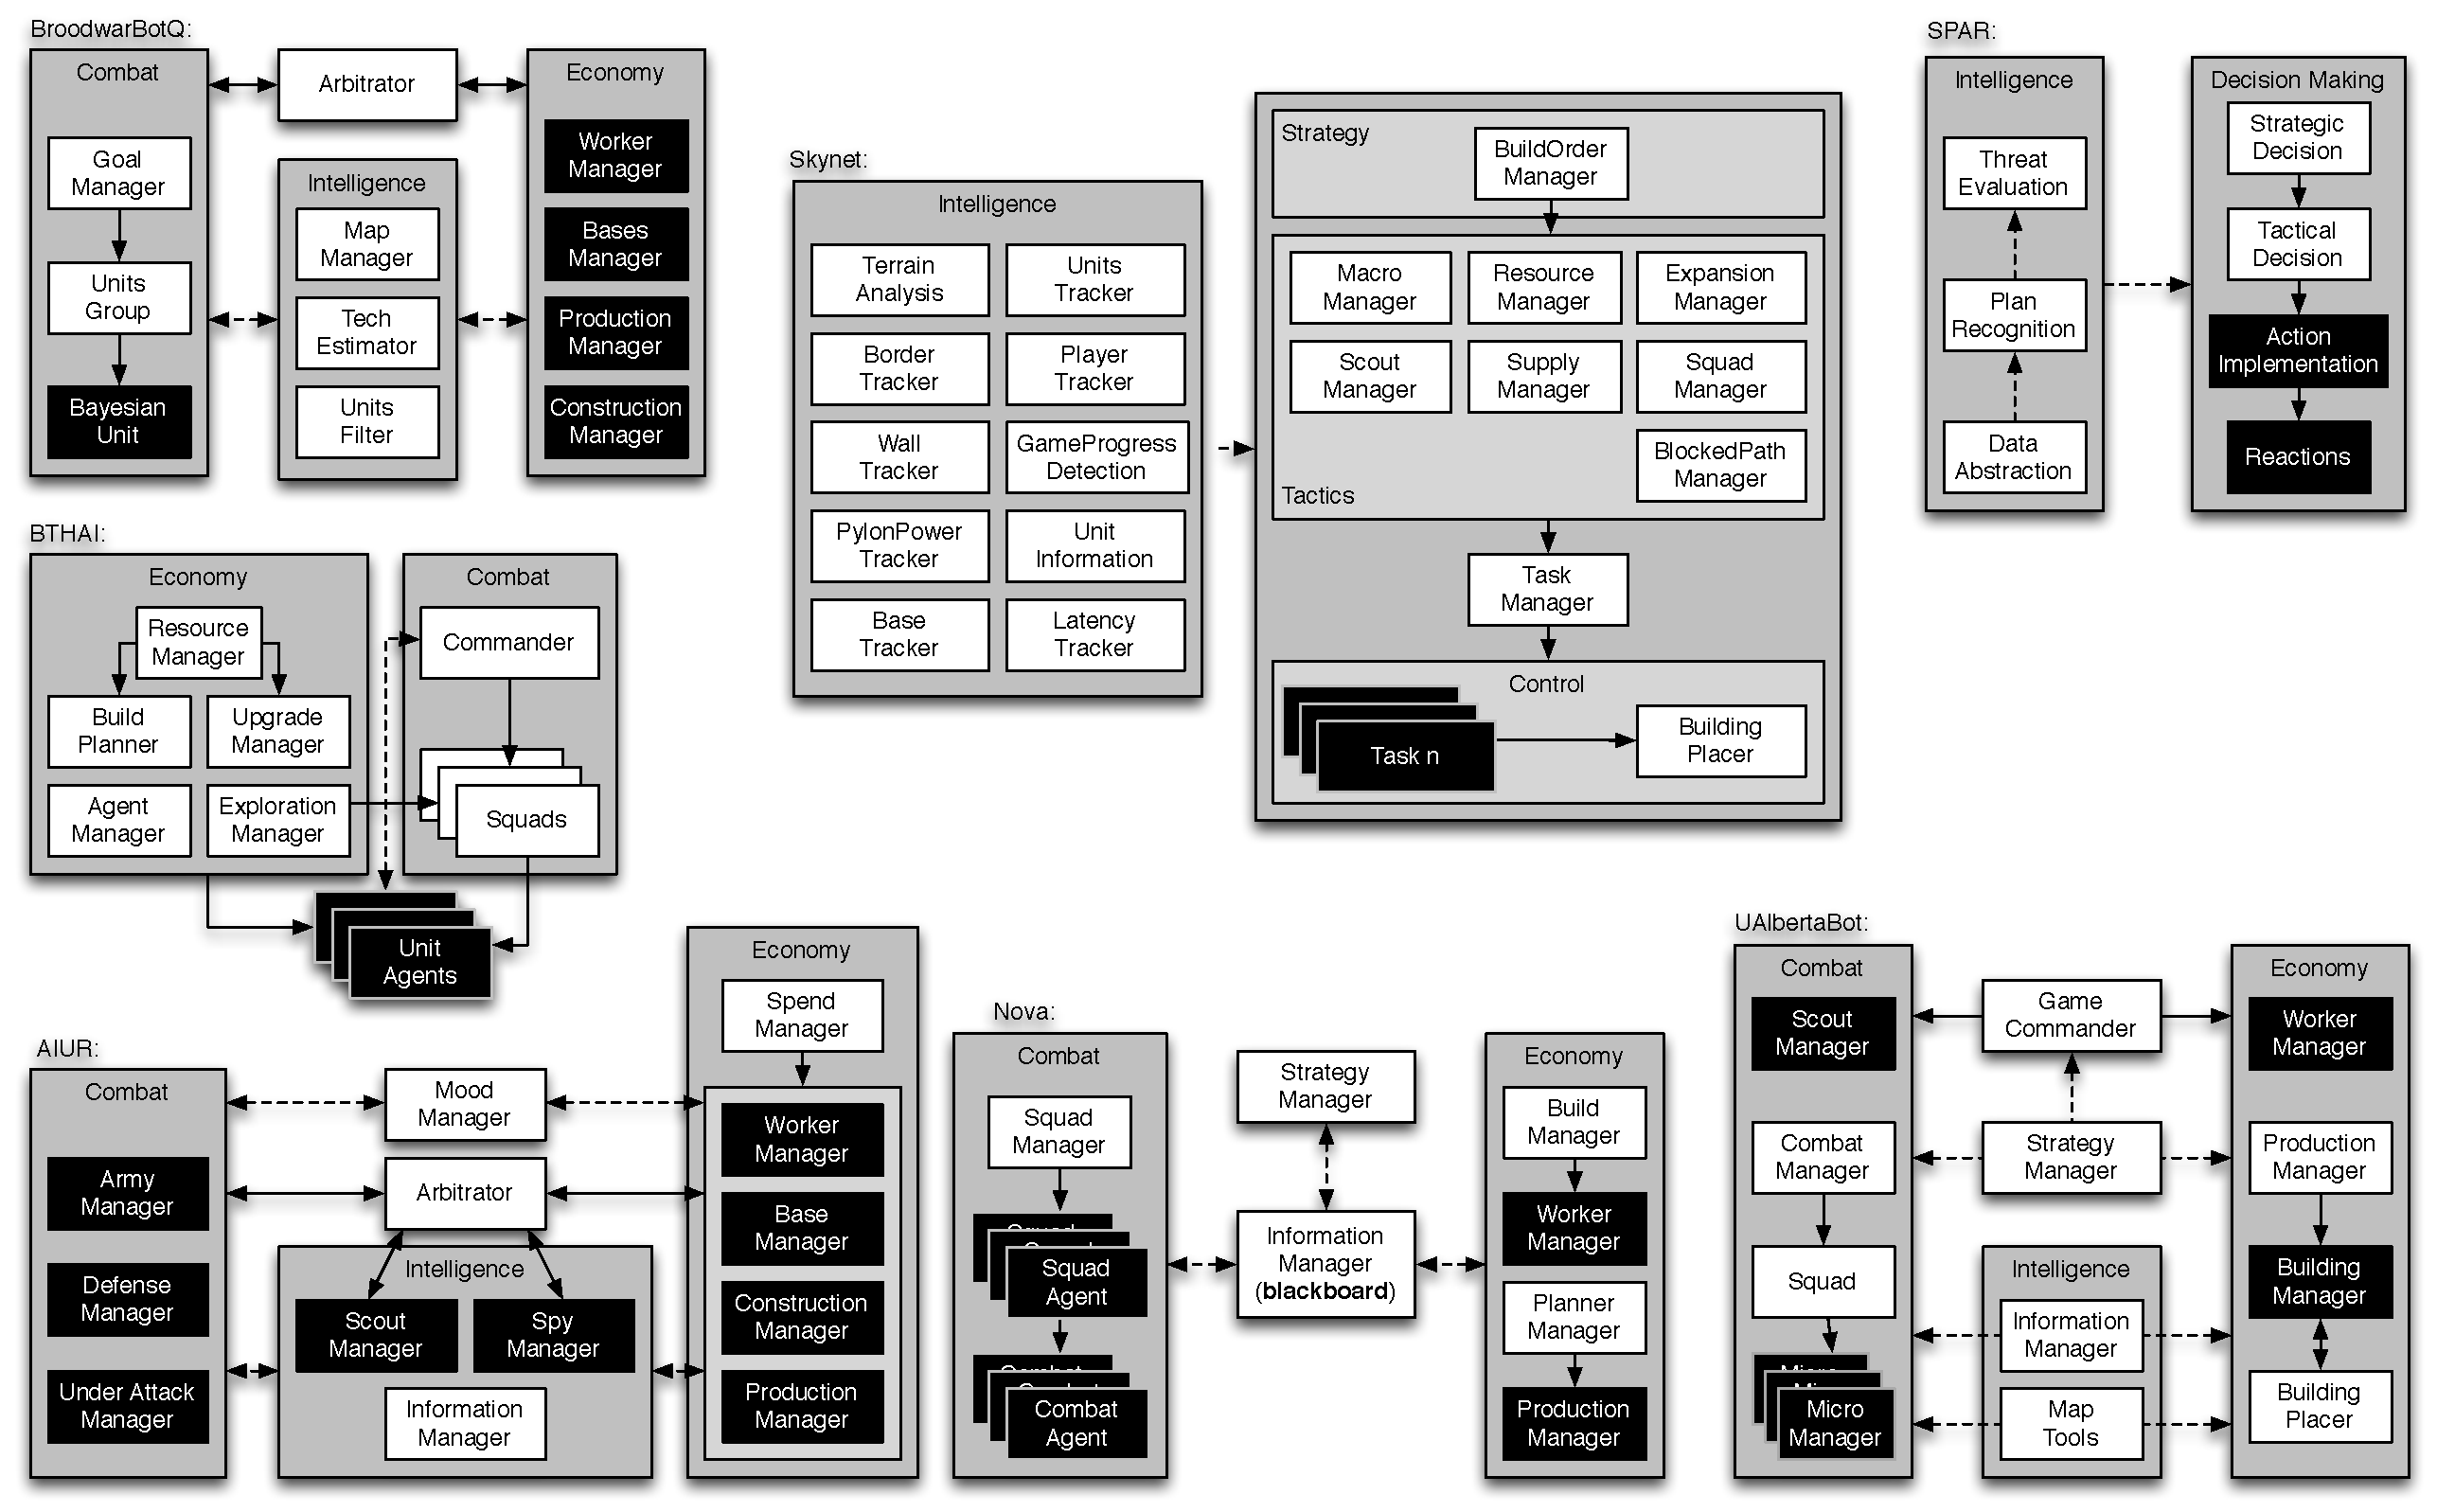
\includegraphics[width=\textwidth]{figures/figure-bot-architectures-wide.pdf}
    \caption{Architecture of 7 StarCraft bots obtained by analyzing their source code. Modules with black background sent commands directly to StarCraft, dashed arrows represent data flow, and solid arrows represent control.}
    \label{fig:bot-architecture}
\end{figure*}

Figure \ref{fig:bot-architecture} shows some representative examples of the architectures used by different bots in the AIIDE and CIG StarCraft AI competitions (see Section \ref{sec:competition}): BroodwarBotQ \cite{SynnaeveMicroCig11}, Nova \cite{uriarte2012kiting}, UAlbertaBot \cite{churchill2011build}, Skynet, SPAR, AIUR, and BTHAI \cite{Hagelback12}. Each box represents an individual module with a clearly defined task (only modules with a black background can send actions directly to StarCraft). Dashed arrows represent data flow, and solid arrows represent control (when a module can command another module to perform some task). For example, we can see how SPAR is divided in two sets of modules: {\em intelligence} and {\em decision making}. Intelligence in SPAR has three modules dedicated to analyze the current situation of the game. Decision making in SPAR is done through four hierarchically organized modules, with the higher-level module ({\em strategic decision}) issuing commands to the next module ({\em tactical decision}), which sends commands to the next module ({\em action implementation}), and so on. Only the two lower-level modules can send actions directly to StarCraft. 

On the other hand, bots such as Nova or BroodwarBotQ (BBQ) only use a hierarchical organization for {\em combat} (controlling the attack units), but use a decentralized organization for the rest of the bot. In Nova and BBQ, there is a collection of modules that control different aspects of the game (workers, production, construction, etc.). These modules can all send actions directly to StarCraft. In Nova those modules coordinate mostly through writing data in a shared blackboard, and in BBQ they coordinate only when they have to use a shared resource (unit) by means of an arbitrator: a bidding market and broker for settling units control, military and civilian groups/task forces bid for units proportionally to their usefulness and the task importance.

By analyzing the structure of these bots, we can see that there are two main tools being used in these integration architectures:

\begin{itemize}
\item {\em Abstraction}: complex tasks can be formulated at different levels of abstraction. For example, playing an RTS game can be seen as issuing individual low-level actions to each of the units in the game, or at a higher level, it can be seen as deploying a specific strategy (e.g. a ``BBS strategy'', or a ``Reaver Drop'' strategy). Some bots, reason at multiple levels of abstraction at the same time, making the task of playing StarCraft simpler. Assuming that each module in the architecture of a bot has a goal and determines some actions to achieve that goal, the actions determined by higher-level modules are considered as the goals of the lower level modules. In this way, each module can focus on reasoning at only one level of abstraction, thus, making the problem easier.

\item {\em Divide-and-conquer}: playing a complex RTS, such as StarCraft, requires performing many conceptually different tasks, such as gathering resources, attacking, placing buildings, etc. Assuming each of these tasks can be performed relatively independently and without interference, we can have one module focusing on each of the tasks independently, thus making the problem easier. 
\end{itemize}

If we imagine the different tasks to perform in a complex RTS game in a two-dimensional plane, where the vertical axis represents abstraction, and the horizontal axis represents the different aspects of the game (combat, resource gathering, etc.), abstraction can be seen as dividing the space with horizontal lines, whereas divide-and-conquer divides the space using vertical lines.

Different bots use different combinations of these two tools. Looking back at Figure \ref{fig:bot-architecture}, we can see the following use of abstraction and divide-in-conquer in the bots:

\begin{itemize}
\item
  BroodwarBotQ\footnote{\url{http://github.com/SnippyHolloW/BroodwarBotQ}}:
  uses  abstraction for  {\em combat}, and  divide-and-conquer for
  {\em economy}  and  {\em intelligence  gathering}. To  avoid  conflicts
  between modules (since  the individual tasks of each  of the modules
  are not completely independent), BBQ uses an arbitrator.
\item  Nova\footnote{\url{http://nova.wolfwork.com/}}:  is similar  in
  design as  BroodwarBotQ, and uses  abstraction for {\em combat},
  and  divide-and-conquer for  {\em economy}.  The differences  are
  that Nova does not have  an arbitrator to resolve conflicts, but has
  a  higher-level   module  ({\em  strategy   manager}),  which  posts
  information to the blackboard that the rest of modules follow (thus,
  making use of abstraction).
\item
  UAlbertaBot\footnote{\url{http://code.google.com/p/ualbertabot/}}:
  also  uses abstraction  in  {\em combat} like  the previous  two
  bots. But it  also uses it in {\em economy}: as  can be seen, the
  production manager sends commands to the building manager, who is in
  charge   of   producing   the   buildings.  This   bot   also   uses
  divide-and-conquer, and  tasks like scouting  and resource gathering
  are managed by separate, independent modules.
\item       Skynet\footnote{\url{http://code.google.com/p/skynetbot/}}:
  makes     extensive     use      of     both     abstraction     and
  divide-and-conquer.  We  can see a  high level module  that issues commands  to a
  series of  tactics modules. The  collection of tactic  modules queue
  {\em  tasks} (that  are analogous  to the  abstract actions  used in
  SPAR).  Each different  task has  a specific  low level  module that
  knows how to  execute it. Thus, Skynet uses  a 3 layered abstraction
  hierarchy,  and uses  divide-and-conquer  in all  levels except  the
  highest.
\item
  SPAR\footnote{\url{http://www.planiart.usherbrooke.ca/projects/spar/}}:
  only uses abstraction. Its high-level module determines the strategy
  to  use,  and  the  tactical  decision  module  divides  it  into  a
  collection  of {\em  abstract  actions}, that  are  executed by  the
  lower-level modules.
\item  AIUR\footnote{\url{http://code.google.com/p/aiurproject/}}:  is
  mainly divide-and-conquer oriented,
  with a  slight abstraction on  {\em economy} due to a  SpendManager deciding
  how  to  spend  and  share  resources  among  Base,  Production  and
  Construction Managers.  At the beginning of a  game, the MoodManager
  initializes  a  ``mood''  which  will  influence  both  tactics  and
  strategy. {\em Combat} is divided into three  independent managers: the
  {\em  Defense Manager},  controlling  military units  when there  is
  nothing special, the {\em  Under Attack Manager}, activated when the
  opponent is attacking our bases,  and the {\em Army Manager}, taking
  control of units when it is time to attack, following a timing given
  by the  current mood. This bot  does not manage however  any kind of
  reactive controls so far.
\item  BTHAI\footnote{\url{http://code.google.com/p/bthai/}}:  uses  a
  two-tier  abstraction hierarchy,  where a  collection  of high-level
  modules command a collection of lower-level agents in charge of each
  of  the units.  At  the high-level,  BTHAI uses  divide-and-conquer,
  having   multiple  high-level  modules   issuing  commands   to  the
  lower-level units.
\end{itemize}

Additionally, except for BTHAI, all other agents use divide-and-conquer at a higher-level bot design and divide all the modules into two or three categories: {\em intelligence gathering} and {\em decision making} (sometimes divided into {\em combat} and {\em economy}).

Some bots  using divide-and-conquer, assume  that each of  the modules
can act independently  and that their actions can  be executed without
interference.  BBQ,  UAlbertaBot and  AIUR, however use  an arbitrator
({\em Game Commander'} in UAlbertaBot) that makes sure that modules do
not send contradictory orders to  the same unit.  However, very little
bots handle  the problem of  how to coordinate resource  usage amongst
modules, for  instance BTHAI uses a  first-come-first-serve policy for
spending resources,  the first module  that requests resources  is the
one that gets them. Nova and Skynet are exceptions, and implement some
rudimentary prioritization based on the high level strategy. Following
available  resources and  timing,  AIUR's {\em  Spend Manager}  orders
Base,  Production   and  Construction  Managers  what   they  have  to
build/produce. It also orders to start tech research and upgrades. The
idea here is not to let the different managers allocate the resources they want, but to do the opposite, that is: finding how the AI can
spend the available money.

One  interesting aspect  of the  seven bots  described above  is that,
while all  of them (except AIUR) are  reactive at the  lower level
(reactive  control), most  if not  all of  them, are  scripted  at the
highest level  of abstraction. BTHAI reads build  and squad formations
from  a  predefined  script,   Nova's  {\em  Strategy  Manager}  is  a
predefined finite-state machine,  BBQ's construction manager reads the
build  order from a  predefined script,  and Skynet's  {\em BuildOrder
  Manager} is basically a predefined script. Such scripts describe the
strategy  that the  bots will  use, however,  such strategy  is always
fixed.   One could see  this pre-scripting  as if  each bot  defined a
``high-level programming language''  to describe StarCraft strategies,
and   the   bots   themselves    are   just   interpreters   of   such
strategy.  Compared  to  current  approaches  for Chess  or  Go,  this
scripting  seems a  rigid and  inflexible,  but responds  to the  much
higher complexity of the  StarCraft game.  An interesting exception to
that  is  UAlbertaBot, which  uses  a  search  algorithm in  the  {\em
  Production  Manager}  to find  near-optimal  build orders.   Another
interesting case is  AIUR, that uses a {\em  Mood Manager} to randomly
pick  a mood among  six (cheese,  rush, aggressive,  defensive, macro,
fast  expand), which  will  influence the  build  order, strategy  and
tactics. % All of  them  scripted so  far,  but build  orders can  been modified but  the Spend Manager, following  available resources.  This mood can change during the game, regarding the opponent behavior.

In conclusion, we can see that there are two basic tools that can be used in an integration architecture: abstraction and divide-and-conquer, which are widely used by the existing StarCraft bots. For space reasons, we do not include an exhaustive comparison of the architectures of all the participating bots. Some other bots have been documented by their authors, such as SCAIL \cite{YoungSCAIL} or QUORUM \cite{young2012evolutionary}.
%This section has focused on discussing the architecture of existing StarCraft bots. 
Let us now focus on their performance.

%\subsection{Individual AI Techniques}\label{sec:techniques}

%{\color{red} TODO}

\section{Recent StarCraft AI Competitions}\label{sec:competition}

This section reviews the results of the recent international competitions on AI for StarCraft. These competitions, typically co-located with scientific conferences, have been possible thanks to the existence of the Brood War Application Programming Interface 
(BWAPI)\footnote{\url{http://code.google.com/p/bwapi/}}, which 
enables replacing the human player interface with C++ code.
%A consequence of this indirect way of integrating new bots is that every machine can only run one custom bot, requiring two computers for a 2-player game.
The following subsections summarize the results of all the StarCraft AI competitions held at the AIIDE (Artificial Intelligence for Interactive Digital Entertainment) and CIG (Computational Intelligence in Games) conferences during the past years. Additionally we analyze the statistics from the StarCraft Bot Ladder, where the best bots play against each other continuously over time. 

\subsection{AIIDE}\label{sec:AIIDE}

Started in 2010, the AIIDE StarCraft AI Competition\footnote{\url{http://www.StarCraftAICompetition.com}} is the most
well known and longest running StarCraft AI Competition in the world. Each year,
AI bots are submitted by competitors to do battle within the retail version of
StarCraft: Brood War, with prizes supplied by Blizzard Entertainment. %This competition has been made possible by the BWAPI StarCraft programming interface, which allows players to write programs which can retrieve game data and issue game commands to StarCraft via an easy to use C++ API.


The first competition in 2010 was organized and run by Ben Weber in the Expressive
Intelligence Studio at University of California, Santa Cruz\footnote{\url{http://eis.ucsc.edu/StarCraftAICompetition}}. 26 total submissions
were received from around the world. As this was the first year of the competition,
and little infrastructure had been created, each game of the tournament was run 
manually on two laptop computers and monitored by hand to record the results. Also,
no persistent data was kept for bots to learn about opponents between matches.

The 2010 competition had 4 different tournament categories in which to compete. Tournament 1
was a flat-terrain unit micro-management battle consisting of four separate unit
composition games. Of the six competitors, FreSCBot won the competition with
Sherbrooke coming in 2nd place. Tournament 2 was another micro-focused game with
non-trivial terrain. Two competitors submitted for this category, with FreSCBot
once again coming in 1st by beating Sherbrooke.

Tournament 3 was a tech-limited StarCraft game on a single known map with no fog-of-war enforced. Players
were only allowed to choose the Protoss race, with no late game units allowed. 8 bots
faced off in this double-elimination tournament with mimicbot taking first place over botnik in the final.
As this was a perfect information variant of StarCraft, mimicbot adopted a strategy of
``mimic its opponent's build order, gaining an economic advantage whenever possible'' which
worked quite well.

Tournament 4 was the complete game of {\em StarCraft: Brood War} with fog-of-war enforced. The tournament
was run with a random pairing double-elimination format with each match being best of 5 games.
Competitors could play as any of the three races, with the only limitations in gameplay
being those that were considered ``cheating'' in the StarCraft community. A map pool of
5 well-known professional maps were announced to competitors in advance, with a random map being chosen for each game.

Results are shown in Table \ref{tab:aiide2010}. The team that won was Overmind\footnote{\url{http://overmind.cs.berkeley.edu}}, from University of California, Berkeley. Using the Zerg race, their
strategy was to defend early aggression with zergling units while amassing mutalisk units,
which they used to contain and eventually defeat their opponents. The mutalisk is a very fast and agile
flying unit which is able to attack while moving with no drawback, which makes them quite a powerful
unit when controlled by a computer. Overmind used a potential-field
based micro-management system to guide their mutalisks, which led them to victory. Krasi0 came in 2nd place
with a standard defensive Terran opening strategy that transitioned into mech play in the late game.

\begin{table}[!t]
\caption{Results of the AIIDE 2010 competition}
\label{tab:aiide2010}
\centering
\begin{tabular}{|c|l|}
\hline
{\bfseries Position} & {\bfseries Bot}\\
\hline
1 & Overmind \\
2 & Krasi0 \\
3 & Chronos \\
\hline
\end{tabular}
\end{table}

In 2011 the University of Alberta hosted the competition, with organization by Michael Buro and
David Churchill\footnote{\url{https://skatgame.net/mburo/sc2011/}}. Due to a lack of entrants in tournament categories 1-3 in the 2010 competition, it was
decided that only the full game category would be played in the 2011 competition. Another important
change in the 2011 competition was the introduction of automated tournament-managing software running
StarCraft games simultaneously on 20 computers, allowing a total of 1170 games to be played in far less
time than the 108 games of the 2010 competition. This increase in games played also allowed the tournament
to switch to a round-robin format, eliminating the ``luck'' factor of the pairings inherent in bracket
style tournaments. The bot that achieved the highest win percentage over the course of the competition would
be determined the winner. Also, the competition became open-source, in an effort not
only to prevent possible cheating, but to promote healthy competition in future tournaments by giving
newcomers and easier entry point by basing their design off of previous bots.

In the  end, Skynet  won the competition  with its solid  Protoss play
(results  are  summarized   in  Table  \ref{tab:aiide2011}).  The  bot
executed one of a small set of strategies randomly at the start of the
match based on the map and the race of the opponent. Skynet would then
amass a  medium to large  sized army and  expand before moving  out to
attack. Good  use of Dragoon (powerful ranged ground unit with clumsy movement) range and  kiting micro-management allowed
it to hold off the early aggression of other bots such as UAlbertaBot,
which came in 2nd.

\begin{table}[!b]
\caption{Results of the AIIDE 2011 competition}
\label{tab:aiide2011}
\centering
\begin{tabular}{|c|l|r|}
\hline
{\bfseries Position} & {\bfseries Bot} & {\bfseries Win \%} \\
\hline
1 & Skynet & 88.9\% \\
2 & UAlbertaBot & 79.4\% \\
3 & AIUR & 70.3\% \\
4 & ItayUndermind & 65.8\% \\
5 & EISBot & 60.6\% \\
\hline
\end{tabular}
\end{table}

UAlbertaBot used an early zealot-rush strategy to take advantage of the power of early game Protoss units. 
It would send out the first zealots that were made and immediately attack the enemy base, using a unit
counting heuristic to determine whether or retreat or keep pushing. Of note is that UAlbertaBot used an
online planning algorithm to construct all of its economic build-orders\cite{churchill2011build}, as no hard-coded build orders
were used. 

AIUR also chose  Protoss, with a strategy that was in between Skynet
and UAlbertaBot in terms of  attack timings.  At that time, AIUR chose
one  mood among  five (leading  to slightly  different  strategies and
tactics) at the  beginning of a game and kept it  until the end. These
five moods were:
\begin{itemize}
\item  Rush:  where  the  bot  tries  early  attacks,  and  have  good
  probabilities to send the two or three first Zealots (basic contact attack ground unit) to harass the
  opponent.
\item Aggressive: where  we have less chance to  perform harasses with
  the first Zealots, and the first attack is usually a bit delayed
  with regard to the Rush mood.
\item Macro: where the AI do not try any early attacks and focus a bit
  more on its economy before attacking.
\item Defense: where the AI  ``turtles'' and wait to have a consequent
  army before running an attack.
\item  Fast expand:  where the  first building  constructed it  a base
  expansion, for a very economical-oriented game.
\end{itemize}
Notice that  build orders are not  fully hard-coded since  they can be
altered by AIUR's Spend Manager.

Of  note  in  these  results  was that  a  rock-paper-scissors  effect
happened among  the top  3 finishers.  Of  the 30 rounds,  Skynet beat
UAlbertaBot 26  times, UAlbertaBot beat  AIUR 29 times, and  AIUR beat
Skynet  19 times.   Another notable  result is  that Overmind  did not
choose  to compete despite  winning the  2010 competition.   After the
competition,  many  bot  programmers  (including  the  Overmind  team)
realized that their  2010 strategy was quite easily  defeated by early
game rushing strategies,  and so they submitted a  Terran bot instead,
called Undermind, which finished in 7th.

After the competition was over, a man vs. machine match was held between the winner (Skynet) and an
ex-professional StarCraft player named Oriol Vinyals. Oriol was a competitor in the 2001 World Cyber
Games StarCraft competition, and though he had been out of practice for a few years was still quite a
good player. The match was arranged to see how well StarCraft AI bots had progressed and to see if
they could actually beat a decent human opponent. 

For the best-of-three match, Oriol chose his races randomly and ended up beating Skynet in a 2-0. 
In the first match, Oriol played Zerg vs. Skynet's Protoss on Python, a four player map. Oriol chose
to start with a fast expansion strategy and transition into two base mutalisk production. Skynet chose
to rush with a few early zealots, which was luckily the best possible choice given Oriol's strategy.
Skynet's initial attack destroyed Oriol's early defenses, and nearly won the game in the first few
minutes, however it then proceeded to send zealots to attack one at a time rather than group up its
units before moving in, which allowed Oriol to catch up. Once Oriol produced his mutalisks, Skynet did
not produce sufficient air defenses and Oriol quickly destroyed Skynet's base. In the second game,
Oril played Terran, again on Python. After holding off early Dragoon pressure from Skynet, Oriol
moved out with a few marines, medics and tanks. Skynet tried to defend with its army of Dragoons,
however due to poor unit targeting decisions it started to attack useless medics after the marines
had died, rather than the tanks. Oriol overcame the Dragoon army and was victorious. Later analysis
of the match concluded that Skynet, while dominant over the other bots, was unable to properly
adapt and transition into a mid-game strategy in game one once its early pressure failed, and in game
two made a key blunder in unit targeting which cost it the game. Humans were still in command.

\begin{table}[!t]
\caption{Results of the AIIDE 2012 competition}
\label{tab:aiide2012}
\centering
\begin{tabular}{|c|l|r|}
\hline
{\bfseries Position} & {\bfseries Bot} & {\bfseries Win \%} \\
\hline
1 & Skynet & 84.4\% \\
2 & AIUR & 72.2\% \\
3 & UAlbertaBot & 68.6\% \\
4 & BroodwarBotQ & 59.1\% \\
5 & AdjutantBot & 52.8\% \\
\hline
\end{tabular}
\end{table}

The University of Alberta also hosted the 2012 competition, with the major difference from the 2011
competition being the addition of persistent storage. Bots could now write information to disk during a
match, and then read the information during other matches, allowing them to adjust strategies based
on previous results. 6 of the 10 entrants used this feature to aid in strategy selection, including the
top 4 finishers. More improvements to the tournament environment also meant that a total of 4240 games
could now be played in the same time period. Results are shown in Table \ref{tab:aiide2012}.

Skynet once  again won  the competition with  its solid  Protoss build
orders  and  good  Dragoon  kiting.   AIUR  and  UAlbertaBot  switched
positions from  the previous  year to come  2nd and  3rd respectively.
Both  AIUR  and UAlbertaBot  used  data  stored  from the  results  of
previous games  to select a strategy for  future matches.  UAlbertaBot
did  this  using  the  UCB  \cite{auer2002finite} algorithm,  while  AIUR  used  a  uniform
distribution  to choose  its  mood before  altering this  distribution
after  some  games  against  the  same  opponent  to  favor  efficient
strategies, achieving  similar results than  UAlbertaBot. Notice that,
compared  to AIIDE 2011,  AIUR proposes  a new  mood, \textit{Cheese},
implementing a  Photon Cannon rush  strategy in order to  surprise the
opponent and  to finish the game  as soon as possible.   The effect of
this strategy selection process can be seen Figure \ref{fig:aiide2012}
which shows bot  win percentages over time.  While  the earlier rounds
of the tournament fluctuated wildly in results, eventually the results
converged to their  final values. One of the main  reasons for this is
due to  the bots  learning which strategies  to use as  the tournament
progressed.

\begin{figure}[t!]
    \centering
    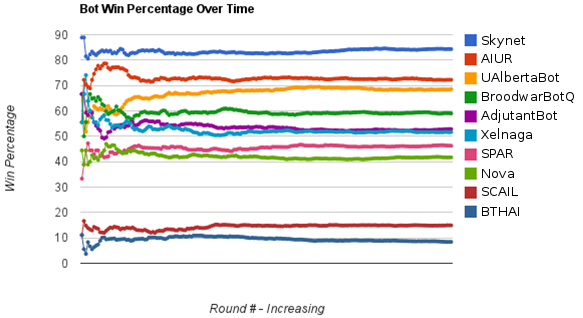
\includegraphics[width=\columnwidth]{figures/aiide2012_v2}
    \caption{Evolution of the win percentage of each bot participating in the AIIDE 2012 competition}
    \label{fig:aiide2012}
\end{figure}








The 2012 man vs. machine match again used the winner of the competition (Skynet), who played against
Mike Lange, also known as Bakuryu. At the time of the match, Bakuryu was an A- ranked Zerg player on ICCup,
and known as one of the best non-Korean Zerg players in the world. Bakuryu was considered much
stronger than Oriol at the time that the match was played, and the results showed that this was true.
In the first game of the best-of-three, Bakuryu made Skynet look quite silly by running around inside
Skynet's base with a small number of zerglings while Skynet's zealots and half of its worked chased
then in vain. After killing off several probes and buying enough time to set up his expansion, he
cleaned up Skynet's army with a flying army of mutalisks. In the second game, Bakuryu contained Skynet
inside its base with a group of zerglings positioned within Skynet's expansion. Skynet then constructed
several Dark Templar and along with some Dragoons and Zealots attacked into Bakuryu's expansion which
was heavily defended, and was crushed almost instantly, allowing Bakuryu's zergling force to finish
off the Protoss base. 

In this match it was shown that the true weakness of state of the art StarCraft AI systems was that
humans are very adept at recognizing scripted behaviors and exploiting them to the fullest. A human
player in Skynet's position in the first game would have realized he was being taken advantage of and
adapted his strategy accordingly, however the inability to put the local context (Bakuryu kiting his
units around his base) into the larger context of the game (that this would delay Skynet until
reinforcements arrived) and then the lack of strategy change to fix the situation led to an easy
victory for the human. These problems remain as some of the main challenges in RTS AI today: to both recognize
the strategy and intent of an opponent's actions, and how to effectively adapt your own strategy to 
overcome them.

All results, videos, and replays from the AIIDE StarCraft AI Competition can be found in \url{http://www.StarCraftAICompetition.com}.
% \footnote{\url{http://www.StarCraftAICompetition.com}}.

\begin{table*}[!t]
\caption{Results of the first round at CIG 2011, held in two brackets.
Qualified for the final round: UAlbertaBot and Skynet (from A), Xelnaga
and BroodwarBotQ (from B, the latter by comparing direct encounters
with BTHAI of which 6:4 were won)}
\label{tab:cig-first-round}
\centering
% bracket A
\begin{tabular}{|c|c|c|l|r|}
\hline
\multicolumn{5}{|c|}{Bracket A} \\ \hline
{\bfseries Position} & {\bfseries Crashes} & {\bfseries Games} & {\bfseries Bot} & {\bfseries Win \%} \\
\hline
A1 & 0 &   40 &  UAlbertaBot & 82.5\% \\
A2 & 1 &     40 &  Skynet   &  77.5\% \\
A3 & 2 &   40 &  AIUR   &  60.0\% \\
A4 & 1 &   40 &  Nova   &  20.0\% \\
A5 & 0 &   40 &  LSAI   &  10.0\%\\
\hline
\end{tabular}
% bracket B
\begin{tabular}{|c|c|c|l|r|}
\hline
\multicolumn{5}{|c|}{Bracket B} \\ \hline
{\bfseries Position} & {\bfseries Crashes} & {\bfseries Games} & {\bfseries Bot} & {\bfseries Win \%} \\
\hline
B1 & 12 &  40 &  Xelnaga &   62.5\%\\
B2 & 3 &   40 &  BroodwarBotQ  &  57.5\%\\
B3 & 0 &   40 &  BTHAI    &  57.5\%\\
B4 & 17 &  40 &  Protoss Beast Jelly  & 42.5\%\\
B5 & 0 &   40 &  EvoBot   &  30.0\%\\
\hline
\end{tabular}
\end{table*}

\subsection{CIG}
\label{sec:cig2011}

An initial attempt to run a StarCraft tournament at the Computational
Intelligence in Games conference (CIG 2010) suffered from technical problems.
These mainly stemmed from the desire to use evolved, largely untested
maps which proved to look interesting but made the submitted bots and the Brood War Terrain Analyzer (BWTA) provided with the BWAPI interface crash
so frequently that it would have been unjustifiable to announce a winner.

At CIG 2011, the tournament was therefore run with a (secret) selection
of maps used in league play, which can be regarded as the most important
difference to the AIIDE tournament that employed a known list of maps.
The competition was organized by Tobias Mahlmann and Mike
Preuss and attracted 10 bots. In addition to the ones discussed in previous
sections (UAlbertaBot, Skynet, AIUR, Nova, BroodwarBotQ, BTHAI), 
the set also contained LSAI, Xelnaga, Protoss Beast Jelly, and EvoBot,
these are shortly described in the following:

\paragraph*{LSAI (Zerg)} utilizes a heavily modified BWSAL\footnote{\url{https://code.google.com/p/bwsal/}} to divide management
 of the units to different modules that communicate via a centralized information
 module. It works using a simple reactive strategy to try and survive early game
 attacks and macro up to a larger attack force and maintain map control.
 
\paragraph*{Xelnaga (Protoss)} is a modification of the AIUR bot that chooses the 
Dark Templar Opening in order to destroy the enemy base before defenses against
invisible units are available. 

\paragraph*{Protoss Beast Jelly (Protoss)}
always goes for a 5-gate Zealot rush, supported by an effective harvesting 
strategy named power-mining (2 probes are assigned to every mineral patch,
thereby needing 18 probes for 100\% saturation in a normal map, prior
to expanding). Gas is not mined as it is not needed for constructing Zealots.

\paragraph*{EvoBot (Terran)} employs an evolutionary algorithm for obtaining rational
 unit combinations and influence map techniques for deciding the strategic locations. Note
 that this bot was submitted in a very early version, with many of its designed features not
 yet fully ready. 

\subsubsection{First Round}
\label{sec:cig-first-round}

\begin{figure}[t]
	%\vspace*{-1ex}
    \centering
    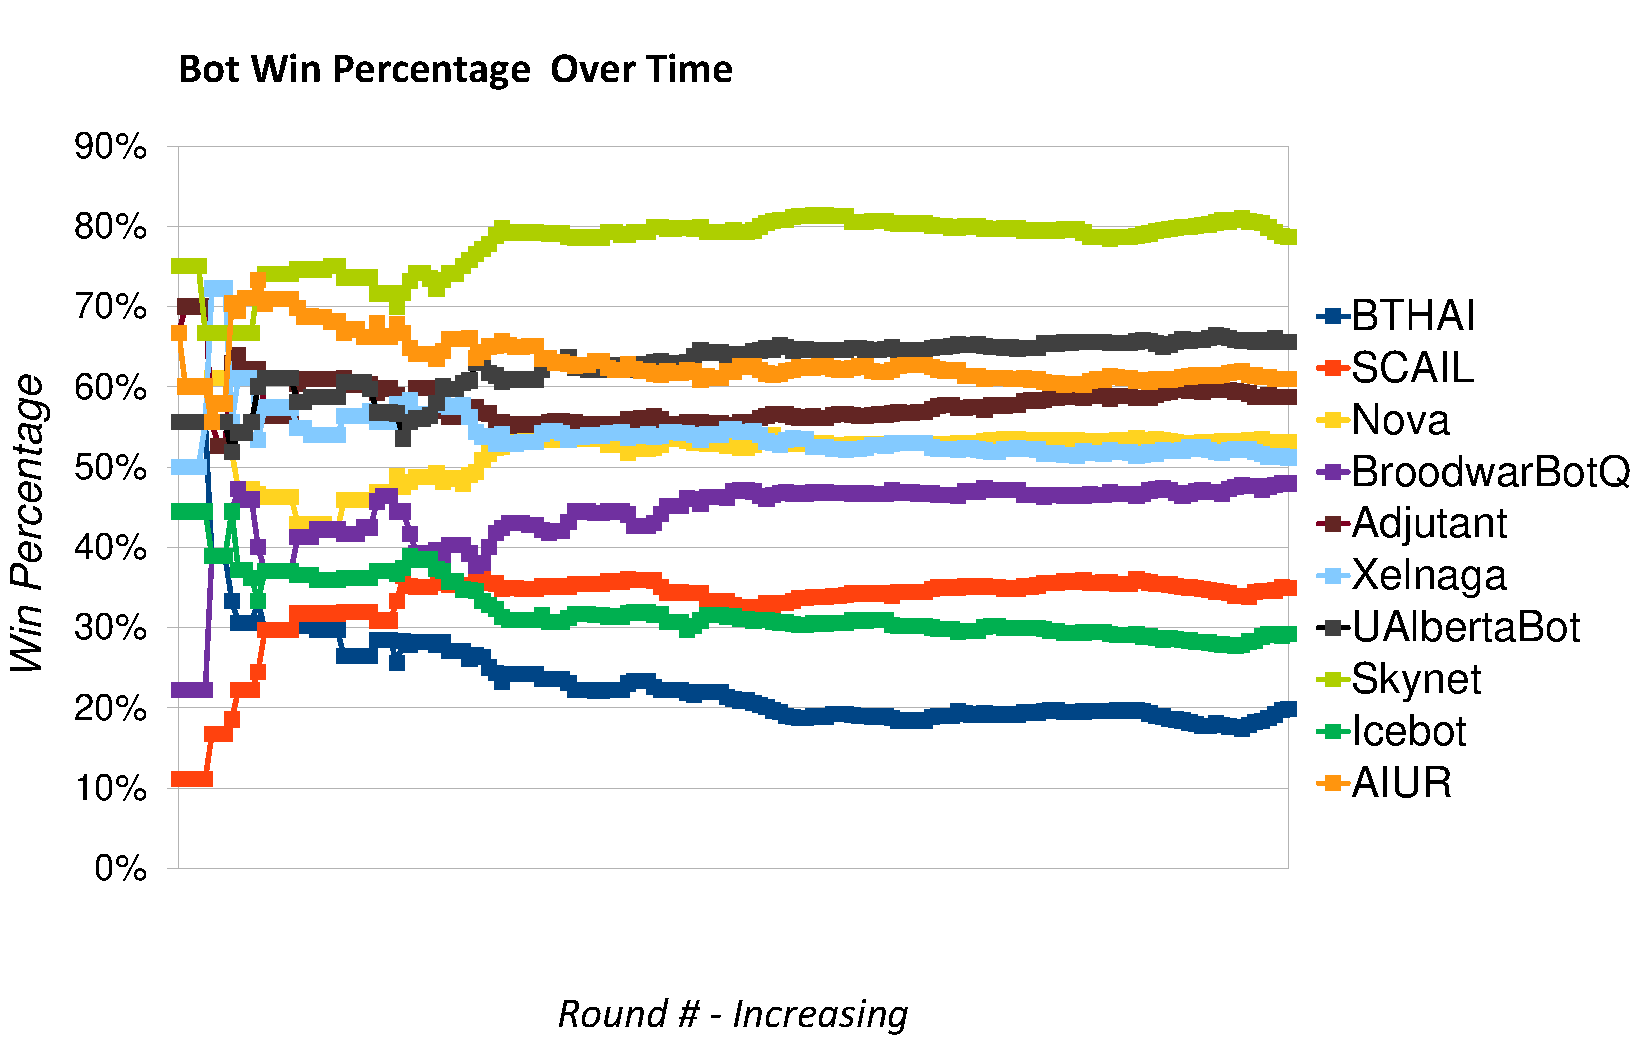
\includegraphics[width=\columnwidth]{figures/cig2012-ResultsRound90.pdf}
	%\vspace*{-1ex}
    \caption{Evolution of the win percentage of each bot participating in the
CIG 2012 competition}
    \label{fig:cig2012-results}
\end{figure}

\begin{figure*}[b]
	%\vspace*{-2ex}
    \centering
    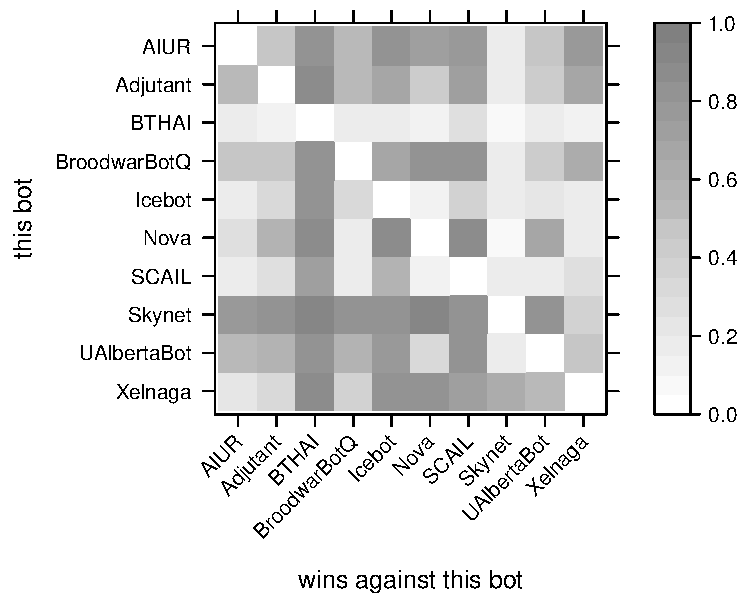
\includegraphics[width=0.32\textwidth]{figures/vstable3.pdf}
    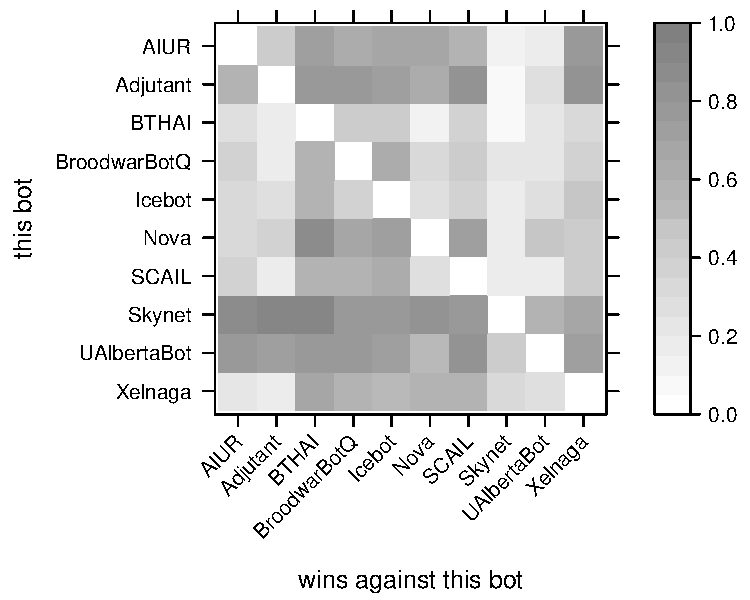
\includegraphics[width=0.32\textwidth]{figures/vstable6.pdf}
    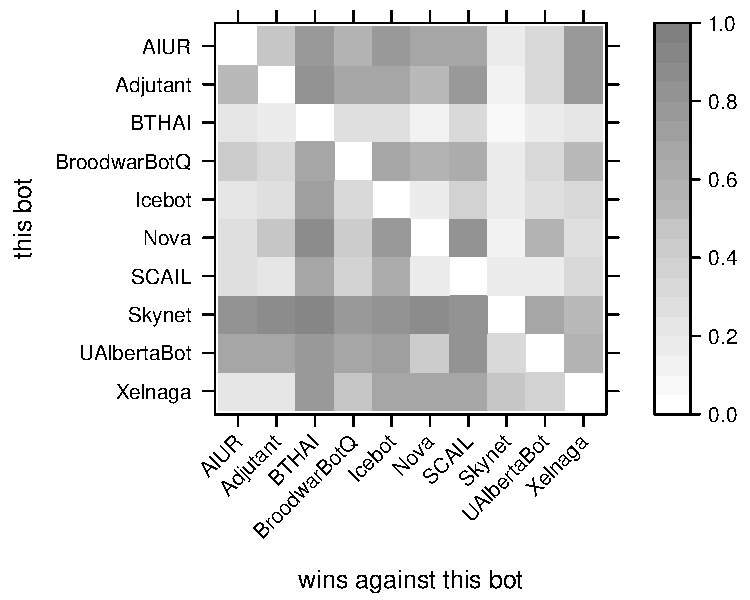
\includegraphics[width=0.32\textwidth]{figures/vstable.pdf}
	%\vspace*{-4ex}
    \caption{Win percentages of CIG 2012 competition, from left
    to right: 3-player maps only, 6-player maps only, all maps.
    Read from line to column, bot in row wins given fraction of
    games against bot in column. For some bots, we find interesting
    differences, e.g. Xelnaga gets worse on 6-player maps, UAlbertaBot
    gets better. Only Xelnaga can reliably beat Skynet, but only on 
    3-player maps}
    \label{fig:cig2012-mapresults}
\end{figure*}

As the CIG competition games were executed manually due to
a lack of available software (the AIIDE program was not yet
available at that time), the organizers separated the ten entries into
two brackets. In each bracket of 5 bots, a round-robin
tournament was held with 10 repetitions per pairing, resulting
in 40 games per bot.
The 5 maps chosen for the first round were selected from the pool
of well-known league play maps found on the internet:
\emph{(2)MatchPoint 1.3}, \emph{(4)Fighting Spirit 1.3}, 
\emph{iCCupdestination 1.1}, \emph{iCCup gaia}, and 
\emph{iCCup great barrier reef}. Each bot pairing played
on every map twice, with switched starting positions.


The two top bots of every bracket qualified
for the final round. Table~\ref{tab:cig-first-round} summarizes
the results.
Note that as BroodwarBotQ and BTHAI have the same number of wins,
their direct encounter was evaluated which accounted 6:4 for the BroodwarBotQ.
The bots going into the final were thus UAlbertaBot, Skynet (from bracket A)
and Xelnaga and BroodwarBotQ (from bracket B). All qualified bots play the
Protoss faction. Most bots proved pretty stable, only Xelnaga and Protoss 
Beast Jelly crashed relatively often (each in more than a quarter of the games). 
Crashing of course resulted in an instant win for the other bot.
In some cases, neither bot was able to finish the other off completely,
so that they went into a passive state. We manually ended such games after
around 15 minutes and assigned victory to the bot that had obtained more
points as indicated on the end game screen.

\begin{table}[!b]
\caption{Results of the CIG 2011 competition}
\label{tab:cig-final-round}
\centering
\begin{tabular}{|c|c|c|l|r|}
\hline
{\bfseries Position} & {\bfseries Crashes} & {\bfseries Games} & {\bfseries Bot} & {\bfseries Win \%} \\
\hline
1 & 0 &  30 &  Skynet       &  86.7\%\\
2 & 0 &  30 &  UAlbertaBot  &  73.3\%\\
3 & 3 &  30 &  Xelnaga      &  36.7\%\\
4 & 2 &  30 &  BroodwarBotQ   &  3.3\%\\
\hline
\end{tabular}
\end{table}



\subsubsection{Final Round}
\label{sec:cig-final-round}

The final round was played in a similar mode as each of the
first round brackets,
using another set of 5 previously unknown maps:
\emph{iCCup lost temple 2.4}, \emph{iCCup rush hour 3.1},
\emph{iCCup swordinthemoon 2.1}, \emph{iCCup yellow 1.1},
and \emph{La\_Mancha 1.1}. 
Letting each pairing play on each map twice again with
switching starting positions resulted in 30 games per bot.
The final results are displayed in table~\ref{tab:cig-final-round},
indicating Skynet as winner and UAlbertaBot as runner-up, being
almost equally strong, and the two other bots as clearly inferior.
The competition setup, documentation and results can be found
in\footnote{\url{http://ls11-www.cs.tu-dortmund.de/rts-competition/StarCraft-cig2011}}.


For CIG 2012, the AIIDE tournament software was employed,
leading to a total of $4050$ games played in $90$ rounds
of round robin. As 6 different maps were used, this means
that each bot played every other on every map 15 times. 
As in the AIIDE competition, writing to and reading from
a bot specific directory was enabled, however, due to 
technical reasons, this feature was constrained to the
computer (of 6) the game was actually run on. We can 
therefore assume that this feature was of minor use for
the CIG competition. The only other difference to the
AIIDE competition was that the used maps were not 
made available to the competitors in advance. 

These maps came in two flavors, namely three 3-player maps:
\emph{Athena-II}, \emph{Neo Moon Glaive}, \emph{Tears of the Moon},
and three 6-player maps:
\emph{Legacy}, \emph{River of Light}, and 
\emph{The Huntress 1.1}. 
We shall note that some bots consistently crashed on one
of the originally considered maps which has thus been replaced.
This is surprising as all maps are well known league play maps
or have been provided with the StarCraft Brood War distribution
itself.
Setup, replays and results for the CIG 2012 competition can be found
here\footnote{\url{http://ls11-www.cs.tu-dortmund.de/rts-competition/StarCraft-cig2012}}.

\begin{table}[t]
\caption{Results of the CIG 2012 competition.}
\label{tab:cig2012}
\centering
\begin{tabular}{|c|l|r|}
\hline
{\bfseries Position} & {\bfseries Bot} & {\bfseries Win \%} \\
\hline
1 & Skynet & 78.3\% \\
2 & UAlbertaBot & 65.2\% \\
3 & AIUR & 60.4\% \\
4 & Adjutant & 58.6\% \\
5 & Nova & 52.4\% \\ 
\hline
\end{tabular}
\end{table}

\begin{figure*}[tb]
    \centering
    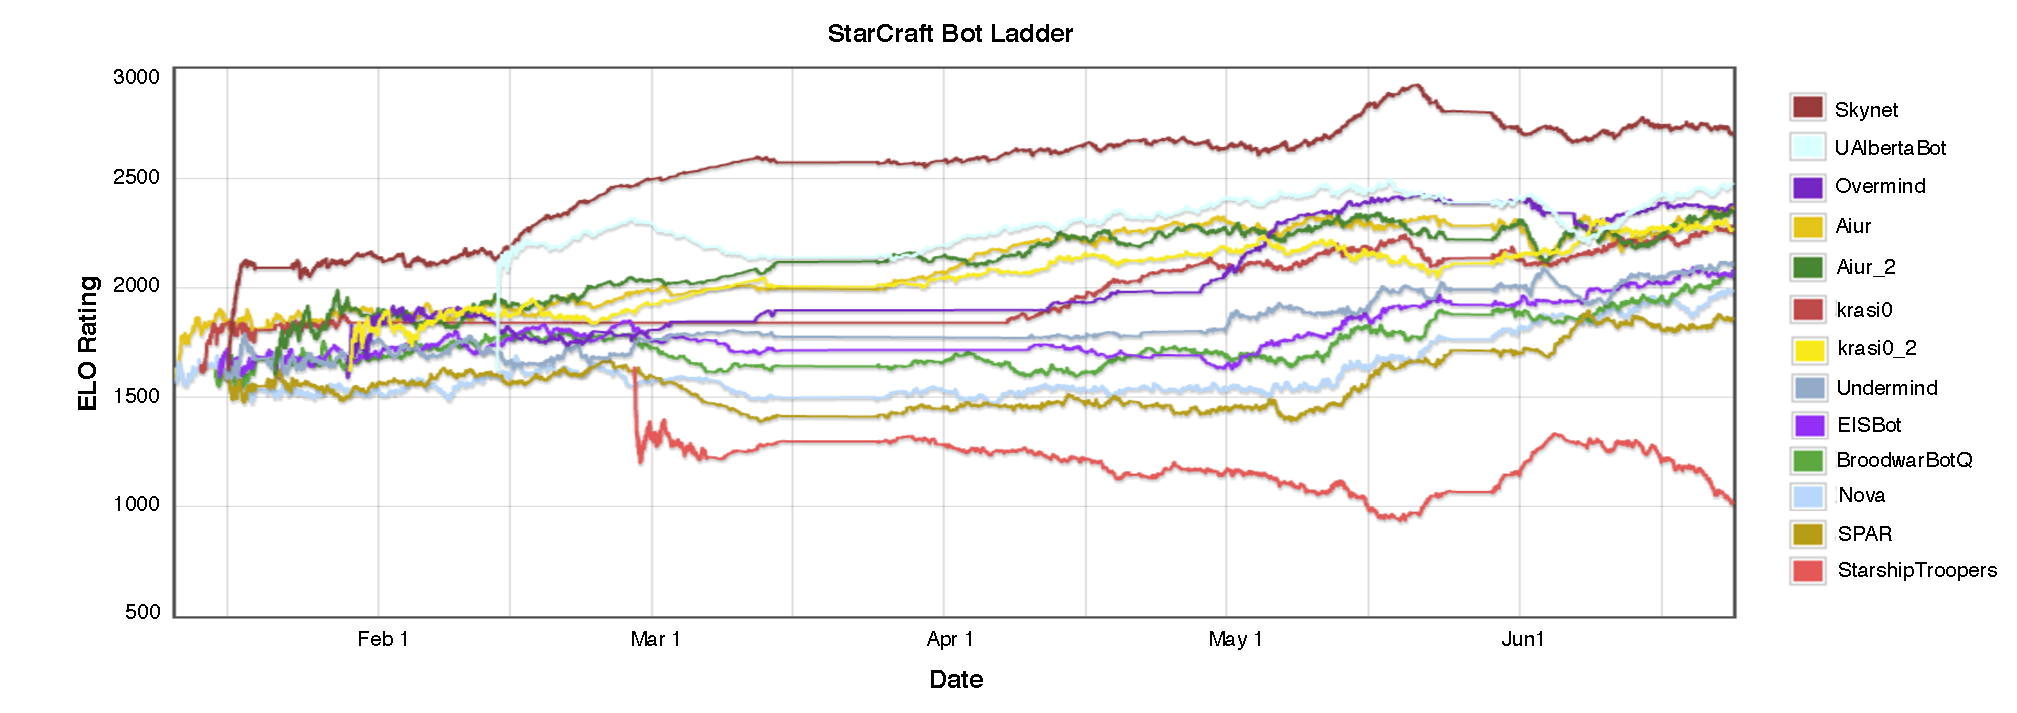
\includegraphics[width=\textwidth]{figures/botLadder1.pdf}
    \caption{Bot's Elo Rating from February 1, 2012 to June 20, 2012}
    \label{fig:botLadder1}
\end{figure*}

\begin{figure*}[tb]
    \centering
    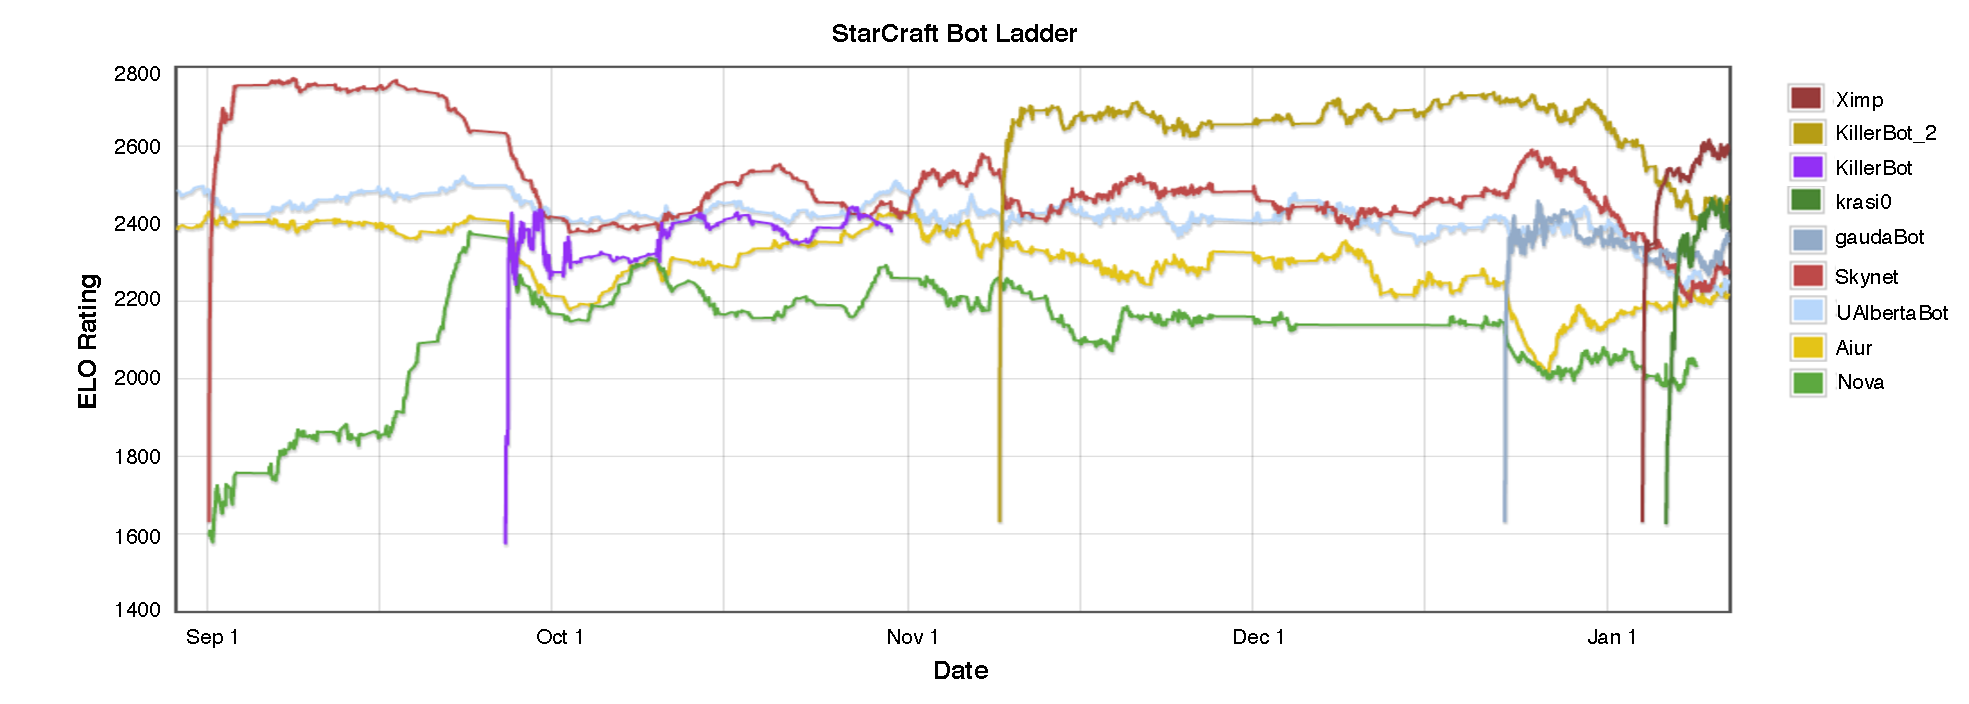
\includegraphics[width=\textwidth]{figures/botLadder2.pdf}
    \caption{Bot's Elo Rating from September 1, 2012 to January 10, 2013}
    \label{fig:botLadder2}
\end{figure*}

The overall results are displayed in table~\ref{tab:cig2012},
and the win rate evolution over time in figure~\ref{fig:cig2012-results}.
These are quite consistent with the results of the AIIDE 2012 competition,
so that we can conclude that the best bots are not very dependent on 
knowing the maps beforehand. However, the bot vs. bot win rates as
displayed in figure~\ref{fig:cig2012-mapresults} show some interesting
trends. On the maps with more possible start points, some bots do 
better than others, namely SCAIL, Adjutant, Nova, and UAlbertaBot,
the latter probably due to its very efficient scouting routine.
Some bots however suffer from the increased uncertainty about
the enemies' position, namely Xelnaga and BroodwarBotQ.

As already observed before in the previously described competitions,
there are also bots who consistently beat top ranked bots but have
severe problems against lower ranked bots. E.g., Xelnaga is especially
strong against Skynet on the 3-player maps (about 70\% wins). Reviewing
the replays led to the assumption that Xelnaga usually tries to attack
Skynet's probes with a dark templar strategy, and often succeeds. 
Nova does very well against the UAlbertaBot, and the replays show
that it sometimes succeeds to lure the probes into its own base, where
they get killed, leading to severe resource problems. However, we cannot
tell how often this happens as this would require to review every single
replay between the 2 bots. Summarizing, most bots seem to have improved,
which becomes clear if the nearly unchanged BTHAI bot is taken as a baseline.
In 2011, it won more than half of its qualifying games, in 2012 it came
out last with around 20\% wins. However, designing a bot in order to 
beat a top bot (as for Xelnaga with Skynet) leads to a very restricted
strategy that often leads to failure if playing against different bots.
Note that in the direct encounter between Xelnaga and AIUR, its ancestor,
Xelnaga looses consistently.

Nevertheless, from the observations we made during the tournament,
we can draw the conclusion that the available bots are still 
very constrained. No bot in the competition played the Zerg race,
which is surprising as the AIIDE 2010 winner (Overmind) did so.
Presumably, implementing a good Zerg strategy is more demanding
than for the Protoss or Terran races. Many bots consistently crashed
when playing against a random race built-in bot for testing, and
also did so when the map size was changed from $128\times 128$ to 
any other. Furthermore, every single bot sometimes failed to finish
off an already beaten opponent, such that the game had to be stopped
after a previously determined maximum time. It also seems that most of
the current bots are not very good at adapting their strategy to the
one of their opponent during a game, or at least (via the read/write
procedure of game information) within a series of games.



\subsection{StarCraft Bot Ladder}\label{sec:ladder}

The StarCraft Bot Ladder is a website\footnote{\url{http://bots-stats.krasi0.com}} where bot versus bot matches are automatized, and are running all the time. This ladder is a great resource for creating data sets (all the game replays are available) and statistics. For bot ranking, the ladder uses an Elo rating system suitable for calculating the \emph{relative skill level} of a bot in two-player games. In the Elo system each player has a numerical rating that gets incremented or decremented some points after each game. The amount of points depends on the difference in the ratings of the players. A player will gain more points by beating a higher-rated player than by beating a lower-rated player. This kind of rating system is widely used in games like chess. This bot ladder compiles different versions of bots from the main worldwide competitions (like AIIDE, CIG or SSCAI\footnote{\url{http://sscaitournament.com}}), even some independent or ``under construction'' bots. Therefore, it is a very good resource to test the performance of new bots against the current state of the art in StarCraft bots before participating in the official competitions.

Figure \ref{fig:botLadder1} shows the Elo rating of the bots in the ladder during the first half year of 2012. The ranking is practically equal than the AIIDE 2011 competition, showing the lack of adaptability of the current bots. We can notice these more extremely in Figure \ref{fig:botLadder2} for the second half year of 2012. During this period new bots were introduced in the ladder. We can observe how the first version of KillerBot made a huge impact on Skynet ranking and finally, the second version of KillerBot quickly became the best bot for more than one month (again we can see how the rest of the bots aren't able to adapt and the ranking doesn't change so much). And finally, in January, the Ximp bot appears with a new strategy that overcomes the rest of the bots. Both KillerBot and Ximp use hard-coded strategies without any kind of adaptation capabilities. However, they implement strategies that no other bot has a counter for, and thus manage to win a very large percentage of games. This points out, once again, that one of the major open challenges in RTS game AI is how achieving adaptive strategies, that can recognize the opponent's intentions, and select an adequate response.


\subsection{Adaptation Analysis}

One of the major conclusions from the results of the StarCraft competitions is the lack of adaptation of bots.  Some switch between different build-orders, but do not fully adapt their strategy. No bot is capable of observing the opponent and autonomously synthesize a good plan from scratch to counter the opponent strategy. In this section we analyzed this claim quantitatively using the tools of \cite{SynnaeveOpeningCig11}. We analyzed the replays from the 2011 and 2012 AIIDE competitions (shown in Figures \ref{fig:aiide2011-botopenings} and \ref{fig:aiide2012-botopenings} respectively). We analyzed the way bots choose their openings depending on which other bot they are playing against. Given that there is no dominant strategy in StarCraft, and it is necessary to see what the opponent is doing in order to determine the best opening, we would expect bots to change their openings depending on which other bot they are playing (since each bot uses a different strategy, or set of strategies). Using clustering, we identified the most common openings in all the replays from the 2011 and 2012 competitions (each one shown with a different color in the figures). No data is shown for the ItayUnvermind bot, since its opening did not match significantly with any of the ones used in our study (extracted from humans pro-gamers).

Specifically, we identified the following openings (for a better comprehension of strategies, buildings or units of StarCraft, we refer the reader to Teamliquid's wiki\footnote{\url{http://wiki.teamliquid.net/starcraft/Category:Strategies}}):
\begin{itemize}
  \item Protoss openings:
  \begin{itemize}
    \item \emph{two\_gates}: Build two \emph{Gateways} and keep training \emph{Zealots} (basic contact attack ground unit), this is the quickest way to apply pressure.
    \item \emph{fast\_dt}: Produce \emph{Dark Templars} (technologically advanced stealth ground unit) as soon as possible, sacrificing early game power for a technological advance, hard-countered by detectors technology.
    \item \emph{templar}: Train \emph{High Templars} (technologically advanced zone attack unit) as fast as possible, same as above, less deadly but is less easily countered.
    \item \emph{speedzeal}: Train \emph{Zealots} and research attack and speed upgrades as soon as possible, some early game power transitioning into late game tech.
    \item \emph{corsair}: Produce \emph{Corsairs} (air-air flying unit) as soon as possible and then transition into training \emph{Dark Templars} (safe from Zerg's flying detectors thanks to \emph{Corsairs}), \emph{Reavers} (ground artillery unit) or \emph{Dragoons}. Weak early game.
    \item \emph{nony}: Build three \emph{Gateways} and massive training of \emph{Dragoons}. Slower than \emph{two\_gates} but still some early game (ranged) power.
    \item \emph{reaver\_drop}: Train \emph{Reavers} as soon as possible to be able to do drops (air transport of artillery units).
  \end{itemize}
  \item Terran openings:
  \begin{itemize}
    \item \emph{bio}: Produce a large army of \emph{Marines} (basic ranged ground unit) and \emph{Medics} (can heal biological units). Quickest way to apply pressure.
    \item \emph{rax\_fe}: Take the closest ``natural expansion'' as soon as possible. This provides a big economic boost in the mid game by sacrificing some early game power.
    \item \emph{two\_facto}: Build two \emph{Factories} and keep producing \emph{Tanks} (ground artillery unit). Vulnerable while building up to it and then very powerful on ground.
    \item \emph{vultures}: Produce mainly \emph{Vultures} (fast ground ranged unit, excels against small units) and research mines. Quicker to reach (technologically) and build than tanks, can transition into tanks.
    \item \emph{air}: Produce \emph{Wraiths} (ranged flying units) as soon as possible for an air attack. Vulnerable to anti-air openings or quick rushes.
    \item \emph{drop}: Train \emph{Dropships} (flying transports) as soon as possible to be able to do (mostly tanks or marines) drops, leveraging efficient tactics.
  \end{itemize}
  \item Zerg openings:
  \begin{itemize}
    \item \emph{speedlings}: Train \emph{Zerlings} (basic cheap, fast, ground contact attack unit) and research speed upgrade as soon as possible. Quickest way to apply pressure.
    \item \emph{fast\_mutas}: Produce mainly \emph{Mutalisks} (ranged flying units). Vulnerable in the early game while gathering gas and researching the technology.
    \item \emph{mutas}: Expand two times for a stronger economy before massive training of \emph{Mutalisks}. Slower but more powerful build-up than above.
    \item \emph{lurkers}: Train \emph{Lurkers} (ground, stealth artillery unit) as soon as possible to benefit from their (advanced technology) zone attack and cloak ability. 
    \item \emph{hydras}: Massive production of \emph{Hydralisks} (ground ranged unit). Much quicker to reach technologically than \emph{Lurkers} and can transition into them.
  \end{itemize}
\end{itemize}

As the figures show, the top three ranked bots in the competition (Skynet, Aiur and UalbertaBot) do not change their strategy at all depending on their opponent. For example, the Skynet bot (both in 2011 and 2012), always uses the same opening (\emph{two\_gates}), except when playing a Terran opponent, when it uses \emph{nony}. This reflects the trend that the performance of bots is still more dependent on carefully handcrafted and non-adaptive behaviors, than on on-line decision making procedures. This is so, since most of the problems that need to be solved in order to implement such procedures are still open.


\section{Open Questions in RTS Game AI}\label{sec:questions}

\begin{figure*}[tb]
    \centering
    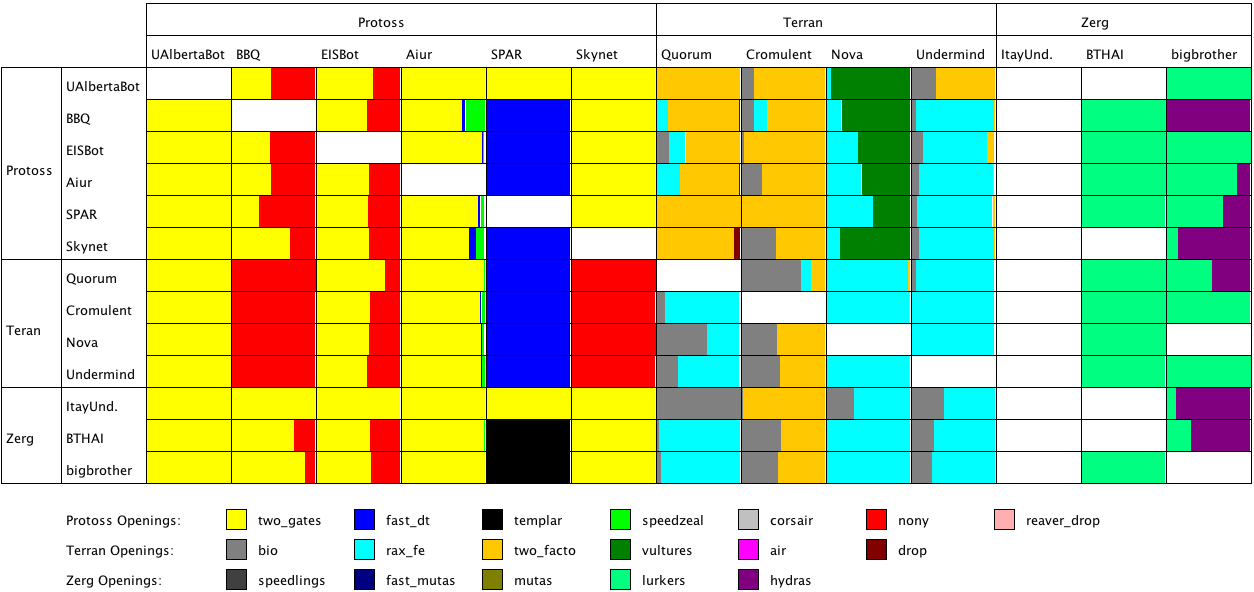
\includegraphics[width=\textwidth]{figures/botopenings2011.png}
    \caption{Distribution of different openings performed by the different bots participating in the AIIDE 2011 competition. For each bot match-up, the colors show the proportion of times that the column bot used a particular opening against the row bot.}
    \label{fig:aiide2011-botopenings}
\end{figure*}

As illustrated in this paper, there is a set of problems in RTS game AI that could be considered mostly solved, of for which we have very good solutions. One example of such problems is pathfinding (mostly solved) or low-scale micro-management (for which we have good solutions). However, there are many other problems for which this is not the case. For example, there is no current StarCraft bot that can come up with its own tactical moves, such as ``unit drops'' in response to an observed opponent strategy. Some bots do drops, but only if this is hard-coded; no bot has the capability of reasoning about the current situation, synthesize a tactical move that involves a ``unit drop'', and determine that this move is the best one in the current situation. This is related to the lack of real-time adversarial planning techniques that scale up to the size required for RTS games. 


\begin{figure*}[tb]
    \centering
    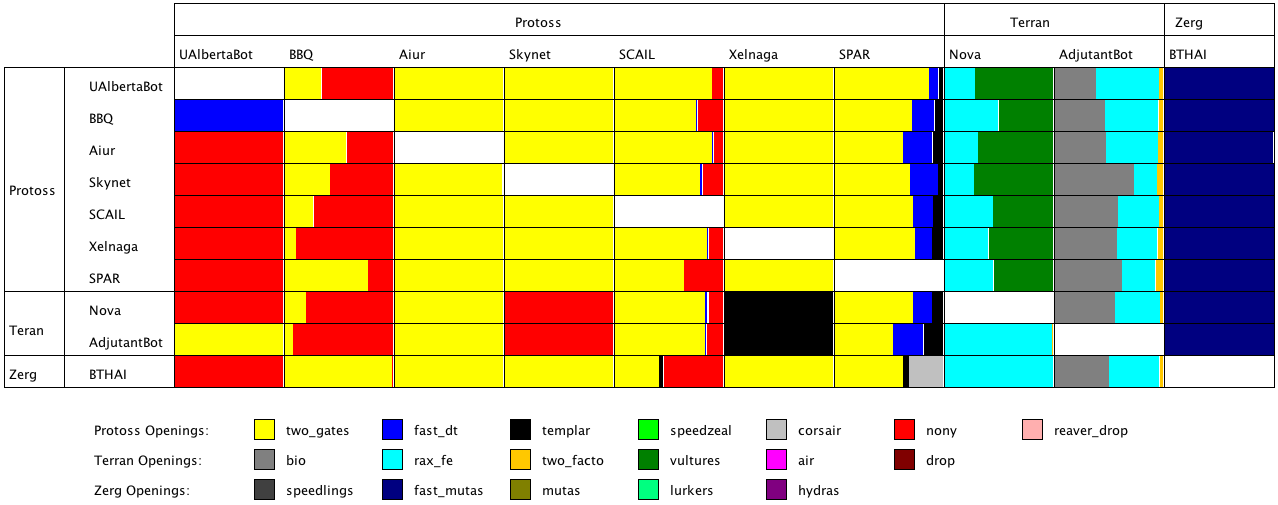
\includegraphics[width=\textwidth]{figures/botopenings2012.png}
    \caption{Distribution of different openings performed by the different bots participating in the AIIDE 2012 competition. For each bot match-up, the colors show the proportion of times that the column bot used a particular opening against the row bot.}
    \label{fig:aiide2012-botopenings}
\end{figure*}

We present here a list of problems that are currently unsolved, grouped in various categories.

\begin{itemize}

\item {\bf Learning and adaptation:}
\begin{itemize}
\item Adaptation to opponent strategy: observing the opponent strategy, and synthesizing an adequate counter strategy. Current bots switch between predefined strategies based on hard-coded preconditions, or based on the performance of each predefined strategy against an opponent in previous games, but no current bot creates new strategies (like Chess or Go playing programs do).
\item Learning from experience in RTS games: how can we make a bot that improves performance over time? Some current bots learn which strategy (out of a predefined set of strategies) is best against a given opponent, but how can we devise learning strategies that can perform more general learning? This has been achieved in classical board games, such as Chess~\cite{tesauro2001comparison}, in the context of game-tree search (by learning the evaluation function). But it's unclear how to do it in RTS games.
\item Learning from observation (from demonstration, or from observing the opponent) in RTS games: how can we learn by observing the game play of other players? Can we devise algorithms that can automatically extract strategies from observation, and later apply them? There has been some work in this direction \cite{OntanonMSR10}, but it is very far from being mature.
\end{itemize}

\item {\bf Planning:}
\begin{itemize}
\item Adversarial planning under real-time constraints: although some solutions for small-scale real-time planning have been recently proposed (such as \cite{churchill2012AIIDE}, based on alpha-beta game-tree search), the problem of large-scale adversarial planning under real-time constraints is still open.
\item Adversarial planning under uncertainty of partially-observable domains: how can we adapt adversarial planning techniques for dealing with uncertainty? This problem has been widely studied in the context of simple games such as back-gammon \cite{tesauro1994td}, or Poker \cite{rubin2011computer}. However, the techniques developed for those domains do not scale to RTS-game scenarios.
\item Adversarial planning with resources: similarly, even if there exist planning algorithms that handle resources (like GRT-R \cite{refanidis2000heuristic}), they cannot scale up to the size of problems needed for RTS games like StarCraft.
\end{itemize}

\item {\bf Integration:}
%\begin{itemize}
%\item 
Multi-scale planning/reasoning: as described in this paper, all the bots developed for the StarCraft AI competitions decompose the problem of playing an RTS game into smaller sub-problems, and then solutions for each of those sub-problems are integrated in to a common architecture to play the game. However, the integration of each of the modules in a unified architecture is still an open problem. For example, how can decisions made at high-level modules be integrated with decisions made at lower-level modules? 
%\end{itemize}

\item {\bf Domain Knowledge: }
%\begin{itemize}
%\item 
We know how to incorporate some aspects of domain knowledge (e.g. build orders) into RTS game playing agents. But, in general, how to incorporate some forms of domain knowledge into algorithms for RTS games is still an open problem. For example, standard techniques to encode strategies for other forms of games, like Behavior Trees, are hard to deploy in RTS games. Is it possible to devise techniques that can automatically mine the existing collections of domain knowledge for an RTS game like StarCraft, and incorporate it into the bot? An initial exploration of this idea was carried out by Branavan et al. \cite{branavan2011learning}.
%\end{itemize}
\end{itemize}



%\section{Empirical Evidence of What is Missing in Existing Bots}\label{sec:experiments}
%
%{\color{blue}
%Here, whatever experiments we want to include to support which aspects of RTS Game AI require more work.
%}

\section{Conclusions}\label{sec:conclusions}

As the list in the previous section indicates, Real-Time Strategy games are an excellent testbed for AI techniques, which pose a very large list of open problems. As Section \ref{sec:competition} has shown, the current top performing programs to play RTS games such as StarCraft still rely mainly on hard-coded strategies. It is still possible to perform strongly, or even win, one of these competitions simply by finding a hard-coded strategy that no other bot has a predefined counter-strategy for. Additionally, good human players are still clearly superior to the best computer programs. From an industry point of view, one additional challenge is to make bots more believable to play against, and thus, more fun for human players (this includes, for example, doing scouting, instead of cheating and having full information of the game state).

One of the main goals of this paper is to provide a centralized and unified overview to the research being done in the area of RTS game AI. To that end, in this paper we have  highlighted the existing challenges in RTS games, from an AI point of view, and surveyed the recent advances towards addressing these challenges with a focus on StarCraft (which has emerged as a unified test-bed). Given that playing an RTS game is a very challenging task, researchers tend to divide such task into smaller tasks, which can be individually addressed by AI techniques. We have also surveyed the different task subdivisions used in some of the top StarCraft-playing programs, highlighting advantages and disadvantages. Additionally, we have presented an analysis of the results of the different StarCraft AI competitions, highlighting strengths and weaknesses of each of the bots. Finally, we have closed the paper with a list of specific open research questions for future research.

Real-time strategy games encompass many interesting and complex
sub-problems that are closely related not only to other fields of AI
research, but to real-world problems as well. For example, optimizing assembly line operations in factories is akin to performing build-order optimizations. 
Troop positioning in military conflicts involves the same spatial and
tactical reasoning used in RTS games. Robot navigation in unknown environments requires real-time path-finding and decision making to avoid hitting obstacles.
All of these issues mentioned in this paper must are being tackled by
the real-time strategy game AI community, and in doing so we will not
only be improving techniques for writing tournament-winning bots, but
for advance the state of the art for many other fields as well.


%As argued before, addressing these open research questions would not just lead to better RTS game playing bots, but would provide means to improve many other complex AI components, not solely focusing on games. This would apply to many areas that are in need of real-time decision components working under uncertainty in the form of incomplete and/or noisy information, such as  e.g. robotics and assistance systems.
%bring significant advances to many other areas of artificial intelligence. This is so because RTS games embody many characteristics of many other problems appearing in many areas of AI (such as robotics, multiagent systems, etc.).  




%\section*{Acknowledgments} {\color{blue} This research is partially funded by projects ... and ... . }



% Can use something like this to put references on a page
% by themselves when using endfloat and the captionsoff option.
\ifCLASSOPTIONcaptionsoff
  \newpage
\fi

%\begin{thebibliography}{1}
%\end{thebibliography}
\bibliographystyle{IEEEtran}                                                    
\bibliography{survey}

%\begin{IEEEbiographynophoto}{FirstName LastName}
%Biography text here.
%\end{IEEEbiographynophoto}

%\begin{IEEEbiography}[{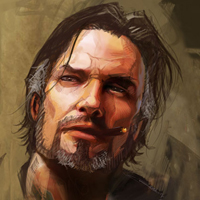
\includegraphics[width=2cm, keepaspectratio]{jim.jpg}}]{Jim Raynor}
%Jim Raynor was a Confederate marshal on Mar Sara at the time of the first zerg incursions on that world. He is now with Raynor's Raiders Inc.
%\end{IEEEbiography}


%\begin{IEEEbiography}[{\includegraphics[width=2cm, keepaspectratio]{figures/santi.jpg}}]{Santiago Onta\~{n}\'{o}n}

% \begin{IEEEbiographynophoto}{Santiago Onta\~{n}\'{o}n}
% is an assistant professor in the Computer Science Department at Drexel University. His main research interests are game AI, case-based reasoning and machine learning, fields in which he has published more than 90 peer-reviewed papers. He obtained his PhD form the Autonomous University of Barcelona (UAB), Spain. Before joining Drexel University, he held postdoctoral research positions at the Artificial Intelligence Research Institute (IIIA) in Barcelona, Spain, at the Georgia Institute of Technology (GeorgiaTech) in Atlanta, USA, and at the University of Barcelona, Spain.  
% \end{IEEEbiographynophoto}

% \begin{IEEEbiographynophoto}{Alberto Uriarte}
% received the B.S. degree in Computer Science from Autonomous University of Barcelona (UAB), Spain, in 2006 and the M.S. degree in Computer Vision and Artificial Intelligence from Autonomous University of Barcelona (UAB), Spain, in 2011. He is currently pursuing the Ph.D. degree in computer science at Drexel University. His research interest includes game AI, RTS games, multiagents systems, procedural content generation, computational geometry, machine learning and drama management.  
% \end{IEEEbiographynophoto}

% \begin{IEEEbiographynophoto}{Florian Richoux}
%   is an associate  professor at the Laboratory of  Computer Science of
%   the University of Nantes,  France.  His main research field concerns
%   parallel  algorithms for solving  constraint-based problems  and has
%   strong  interests   in  AI,  in  particular  game   AI  and  machine
%   learning. He  obtained his Ph.D. in Theoretical  Computer Science at
%   the {\'E}cole Polytechnique  in 2009 and has been  for three years a
%   CNRS   research  fellow  at   the  Japanese-French   Laboratory  for
%   Informatics of the University of Tokyo, Japan.
% \end{IEEEbiographynophoto}

\end{document}


In his AIIDE 2010 keynote, Chris Jurnet described the technique XXX, implemented by [COMPANY] in the game YYY \cite{gameurl}
